\documentclass[11pt]{article}
\usepackage{amsmath}
\usepackage{graphicx}
\usepackage{hyperref}
\usepackage[utf8]{inputenc}
\usepackage[spanish]{babel}
\usepackage[margin=2cm]{geometry}
\usepackage{amsfonts}
\usepackage{listings}
\usepackage[T1]{fontenc}
\usepackage{float}
\usepackage{subfig}

\title{Práctica Minería de Medios Sociales.}
\author{Curso: 2018/2019. Néstor Rodríguez Vico. DNI: 75573052C - \href{mailto:nrv23@correo.ugr.es}{nrv23@correo.ugr.es}}
\date{\today}


\lstdefinestyle{bash_style}{
	language=bash,
	frame=single,
	xleftmargin=.25in,
	upquote = true,
	basicstyle=\scriptsize,
	breakatwhitespace=false,         
	breaklines=true,                 
	captionpos=b,                    
	keepspaces=true,                 
	numbers=left,                    
	numbersep=5pt,                  
	showspaces=false,                
	showstringspaces=false,
	showtabs=false,                  
	tabsize=2
}

\lstset{style=bash_style}

\begin{document}
\maketitle

\setlength{\belowdisplayskip}{5pt} 
\setlength{\belowdisplayshortskip}{5pt}
\setlength{\abovedisplayskip}{5pt} 
\setlength{\abovedisplayshortskip}{5pt}

\section{Introducción.}

Con una tarea como la de predecir el tiempo de viaje de los taxis, puede ser interesante observar y estudiar la estructura de calles subyacente de la ciudad. El análisis de la red puede permitirnos entender por qué ciertos viajes en taxi toman más tiempo que otros, dadas algunas propiedades básicas de la red. El conjunto de datos (el cual se encuentra en el siguiente enlace: \href{https://www.kaggle.com/crailtap/street-network-of-new-york-in-graphml/}{https://www.kaggle.com/crailtap/street-network-of-new-york-in-graphml/}) usado contiene un gráfico para la red de calles para el área de Manhattan para realizar pruebas rápidas de su análisis. Cada nodo representa unas coordenadas en el mapa y hay una relación entre el nodo \textit{i} y el nodo \textit{j} si hay una ruta entre ambos nodos. Nos encontramos ante una red dirigida ya que, según las normas de circulación, poder ir del punto \textit{i} al punto \textit{j} no garantiza que se pueda ir del punto \textit{j} al punto \textit{i}. Dicha red ha sido obtenida con el software \textit{osmnx} (\href{https://geoffboeing.com/publications/osmnx-complex-street-networks/}{https://geoffboeing.com/publications/osmnx-complex-street-networks/}). \\

Aclaración: se ha usado Gephi para la realización de esta práctica pero, también se ha usado \textit{networkx}, un módulo de Python, para obenter ciertos gráficos y métricas. Los scripts y el código relacionados con esto no se han entregado ya que no es el ámbito de la práctica pero, si fuese necesario, no dude en contactar conmigo y se los mando.

\section{Análisis.}

\subsection{Análisis Básico de la Red.}

Lo primero que vamos a hacer es mostrar la red:

\begin{figure}[H]
	\centering
	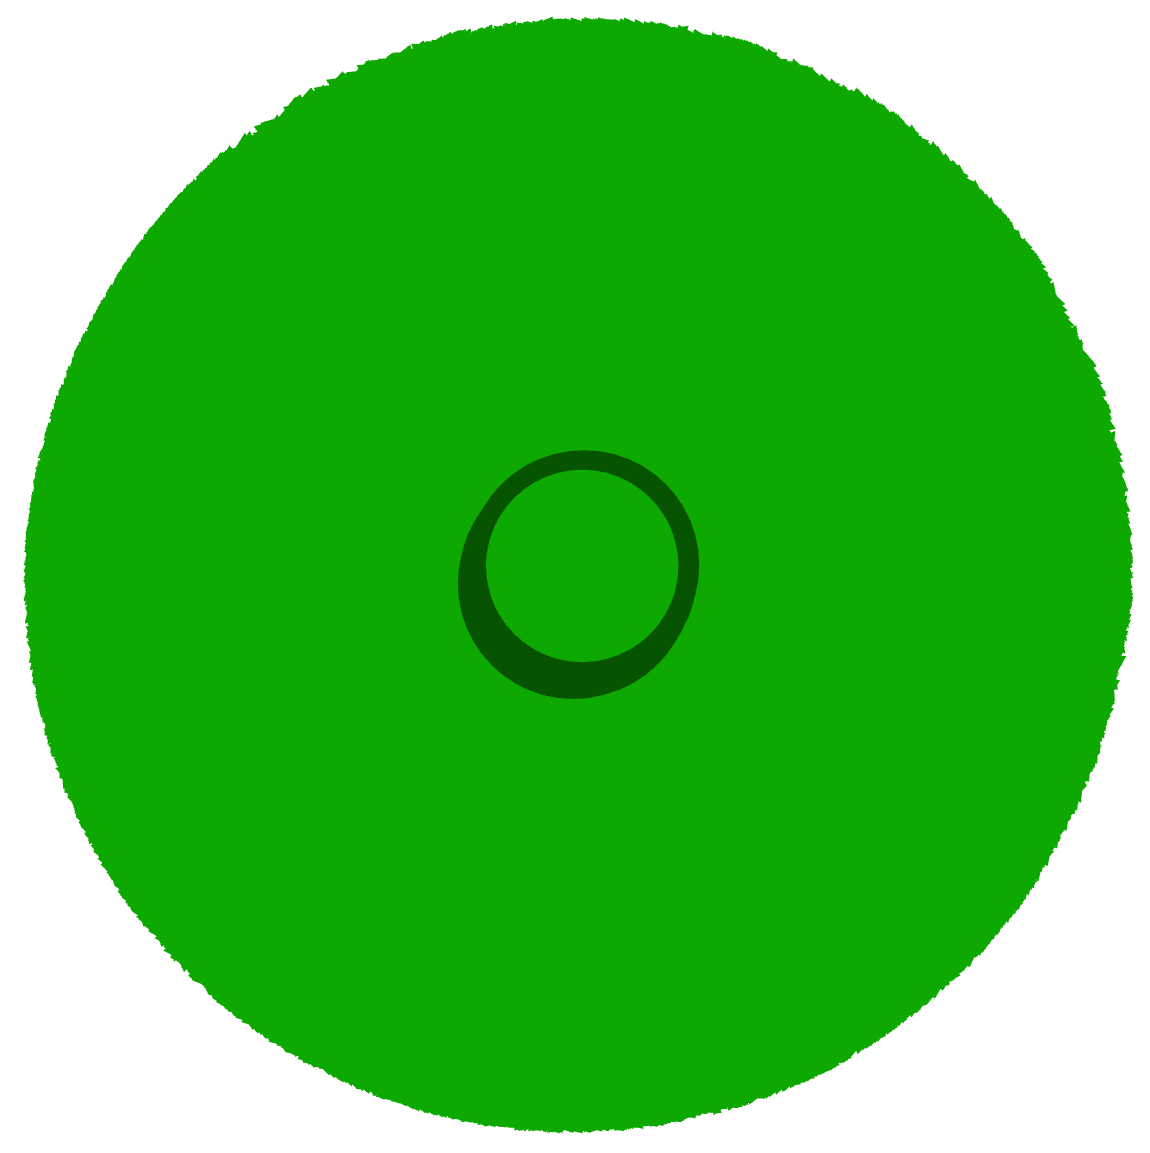
\includegraphics[width=0.4\linewidth]{images/2_1_general.png}
\end{figure}

Parece que no hay nada, pero si ponemos el ratón por encima, podemos ver que hay enlaces y nodos:

\begin{figure}[H]
	\centering
	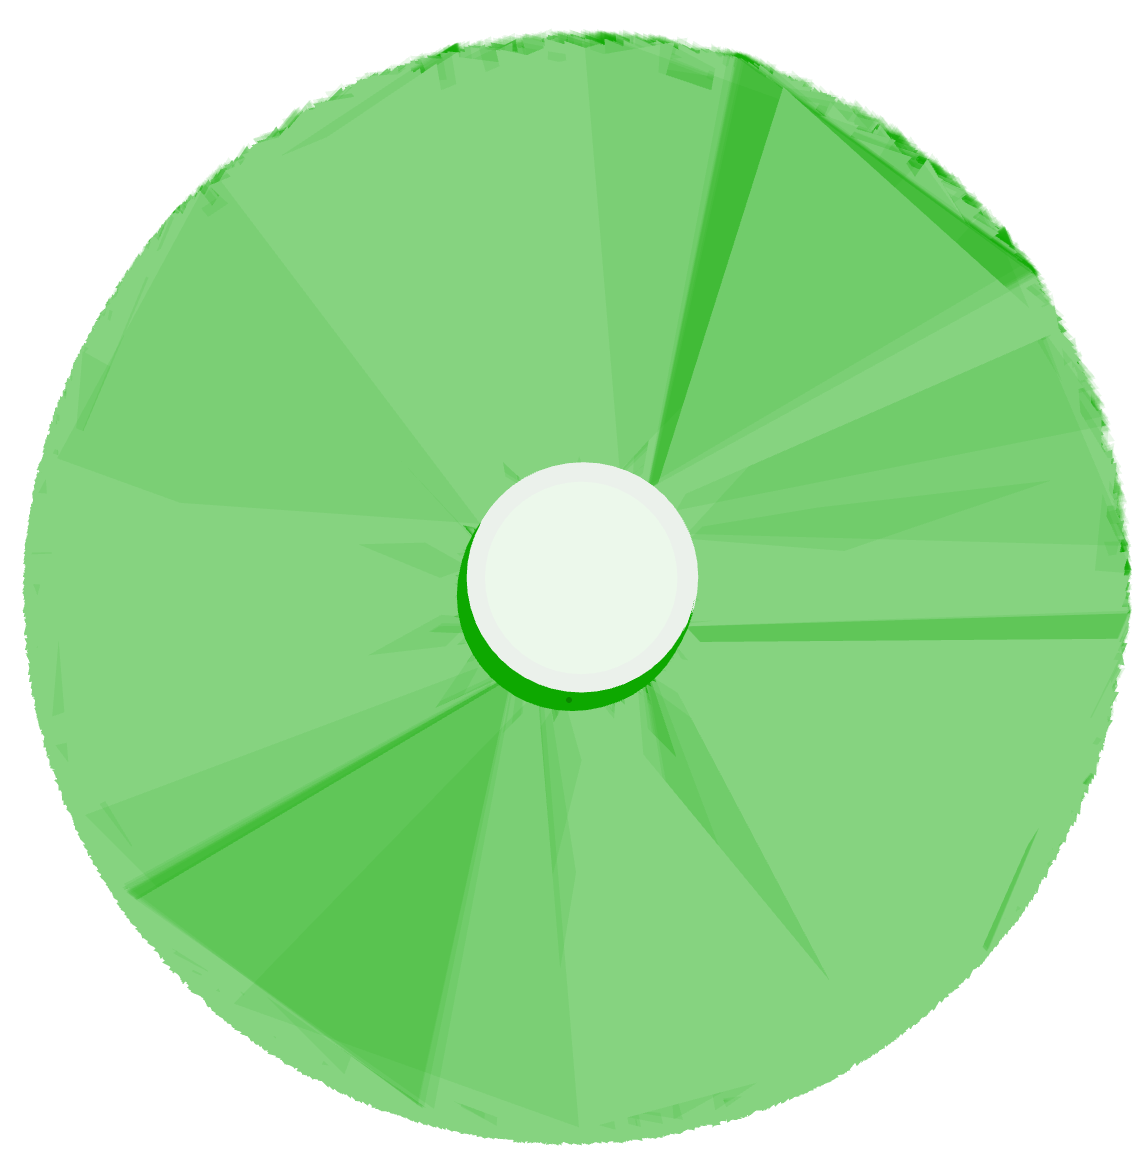
\includegraphics[width=0.4\linewidth]{images/2_1_general_raton.png}
\end{figure}

Para ver la red de una manera más correcta vamos a aplicar el algoritmo \textit{Fruchterman Reingold} y el algoritmos \textit{Force Atlas 2}:

\begin{figure}[H]
	\centering
	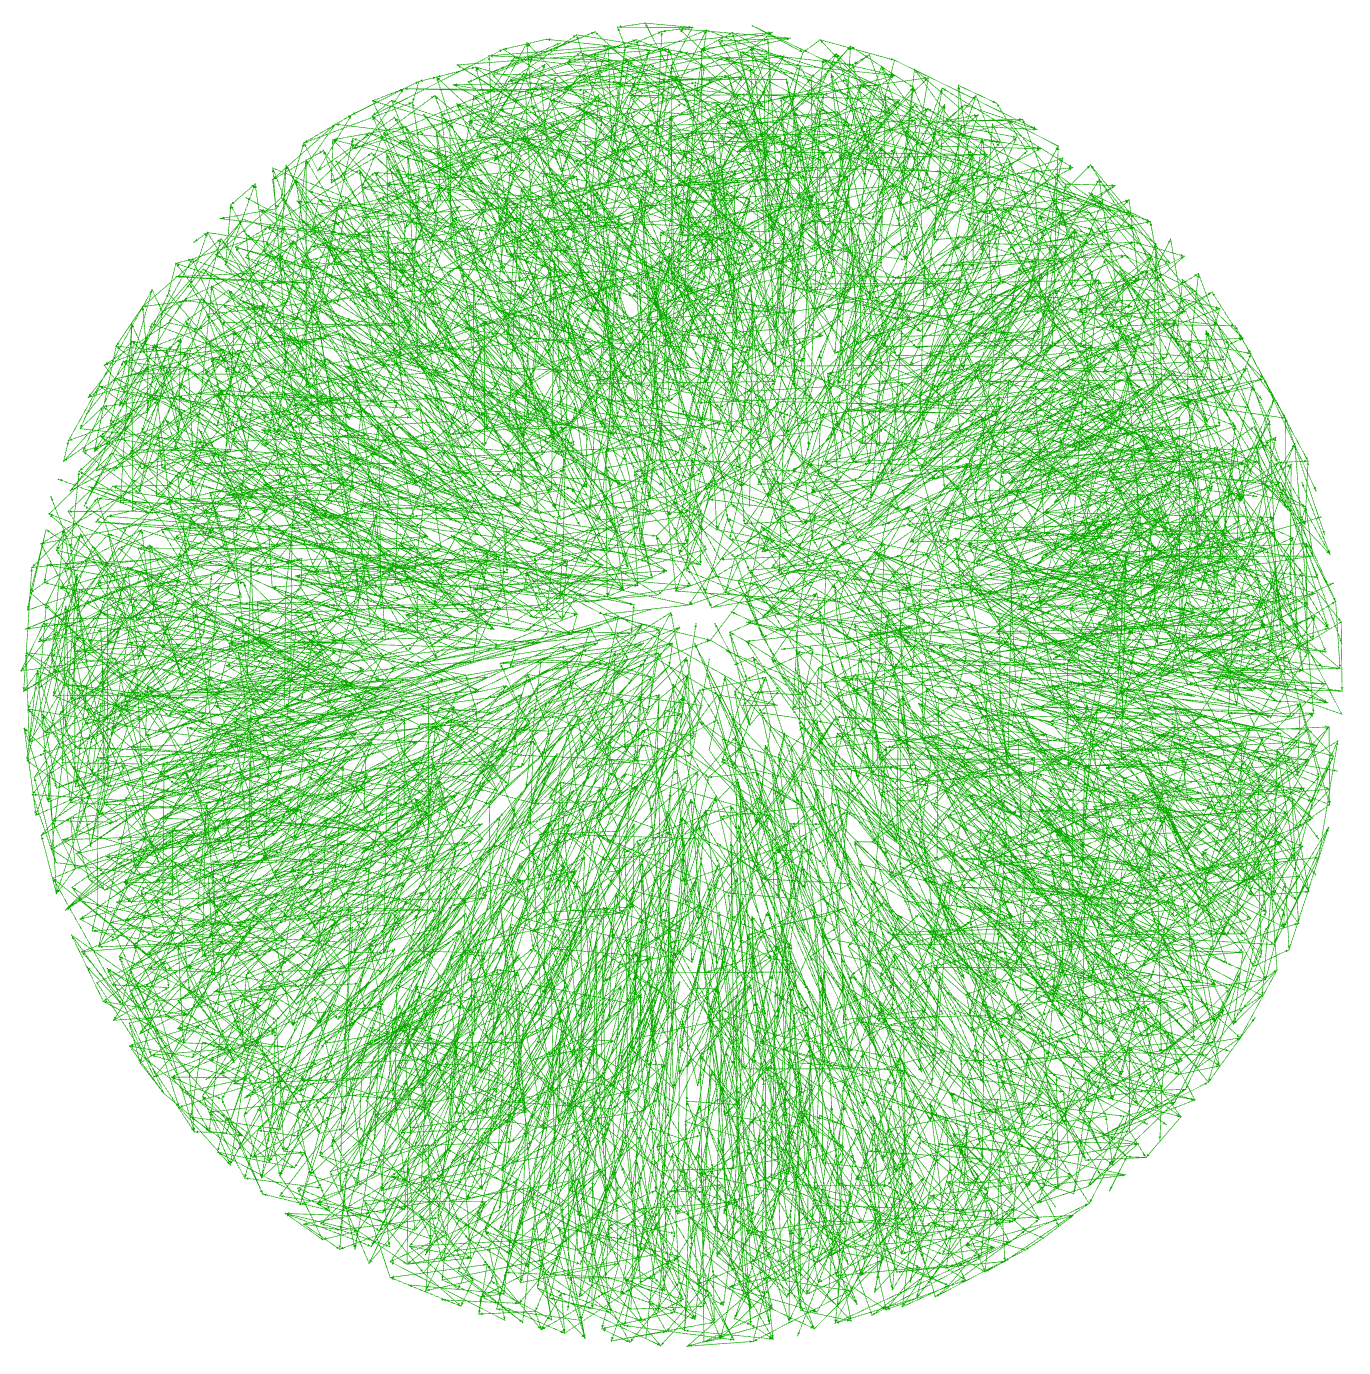
\includegraphics[width=0.7\linewidth]{images/2_1_fr.png}
	\caption{Visualización con \textit{Fruchterman Reingold}.}
\end{figure}

\begin{figure}[H]
	\centering
	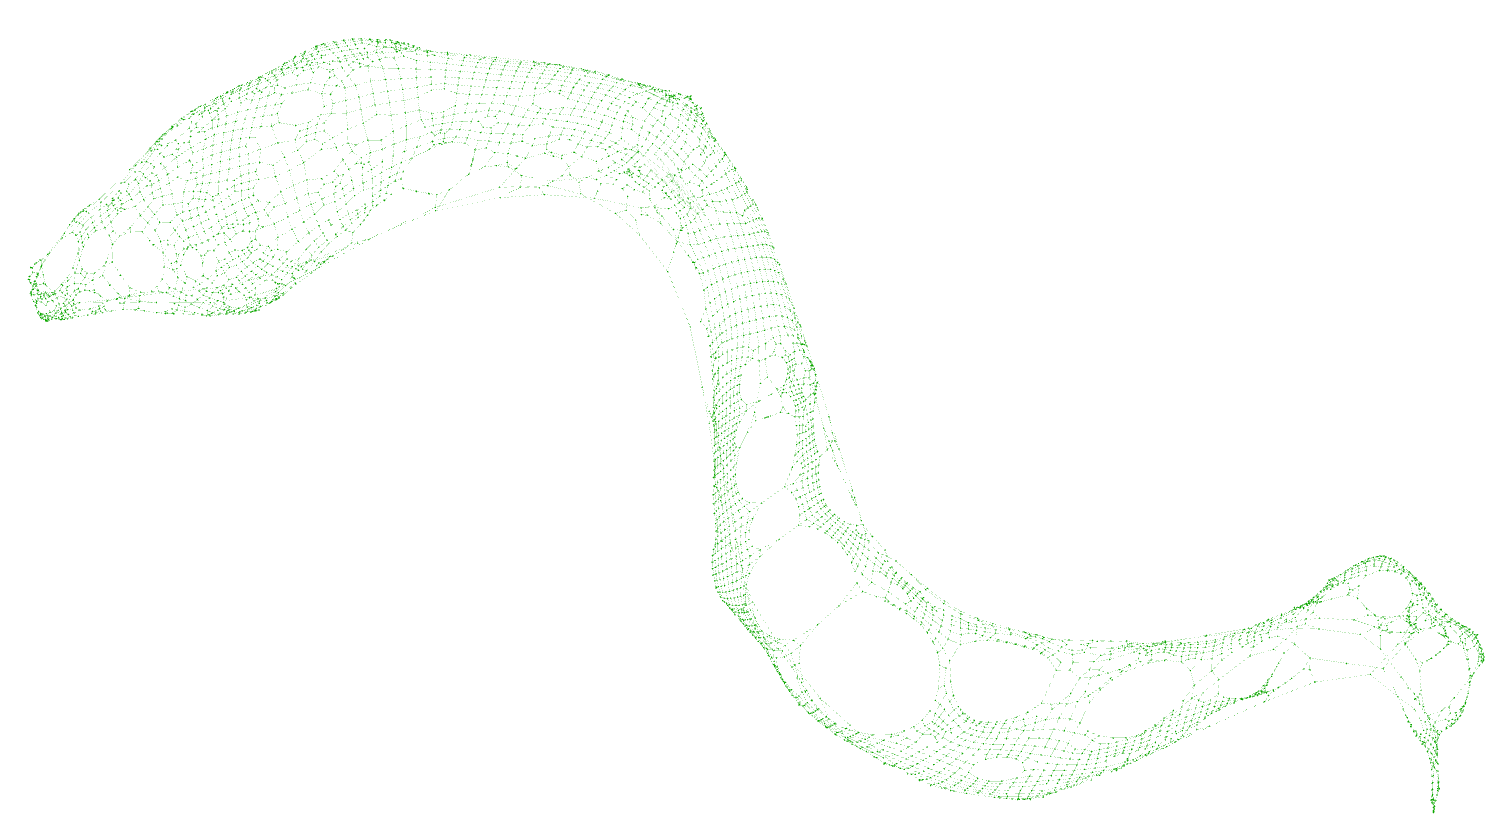
\includegraphics[width=\linewidth]{images/2_1_fa.png}
	\caption{Visualización con \textit{Force Atlas 2}.}
\end{figure}

A continuación, vamos a mostrar una tabla con ciertos valores generales de la red:

\begin{table}[H]
	\centering
	\begin{tabular}{ll}
		\textbf{Número de nodos: N} & 4426 \\
		\textbf{Número de enlaces: L} & 9626 \\
		\textbf{Número máximo de enlaces L$_{max}$ = N * (N - 1)}:  & 19585050 \\
		\textbf{Densidad: D} & 0.0004914 \\
		\textbf{Grado medio: \textless k\textgreater} & 2.175 \\
		\textbf{Diametro: $d_{max}$} & 126 \\
		\textbf{Distancia media: \textless d\textgreater} & 44.826846 \\
		\textbf{Distancia media aleatoria \textless $d_{aleatoria}$\textgreater} & 1.09245 \\
		\textbf{Coef. de clustering medio \textless C\textgreater} & 0.023 \\
		\textbf{Coef. de clustering medio aleatoria \textless $C_{aleatoria}$\textgreater} & 0.491414\\
		\textbf{Número de componentes conexas} &  1\\
		\textbf{Número nodos componente gigante} &  4426\\
		\textbf{Porcentaje con respecto a red total} &  100\%\\
		\textbf{Número enlaces componente gigante} & 9626\\
		\textbf{Porcentaje con respecto a red total} &  100\%
	\end{tabular}
\end{table}

Para calcular la distancia media de una red aleatoria equivalente, he aplicado la siguiente fórmula:

\[<d_{aleatoria}> = \frac{logN}{log <k>} = \frac{log\ 4426}{log\ 2.175} =  1.09245\]

Para calcular el coeficiente de clustering medio de una red aleatoria equivalente, he aplicado la siguiente fórmula:

\[C = \frac{<k>}{N} = \frac{2.175}{4426} = 0.491414\]

A continuación, vamos a ver la distribución de grados:

\begin{figure}[H]
	\centering
	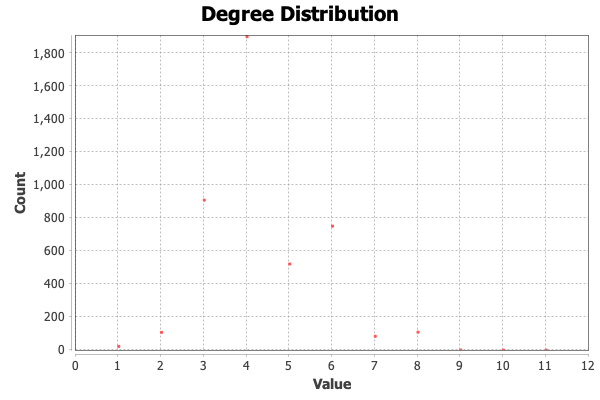
\includegraphics[scale=0.35]{images/2_1_degree-distribution.png}
\end{figure}

Dado que se trata una red dirigida, vamos a ver las distribuciones de grado tanto de entrada como se salida:

\begin{table}[H]
	\centering
	\begin{tabular}{cc}
		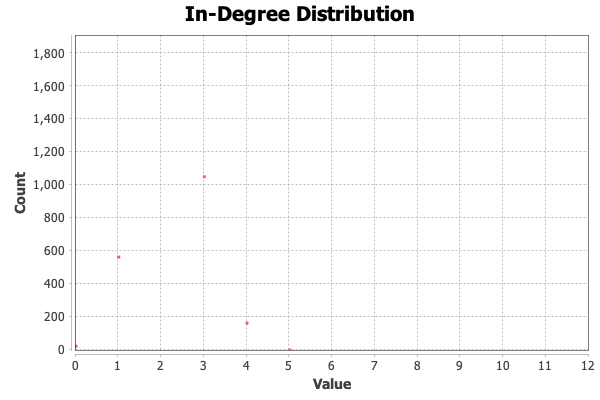
\includegraphics[scale=0.35]{images/2_1_indegree-distribution.png} & 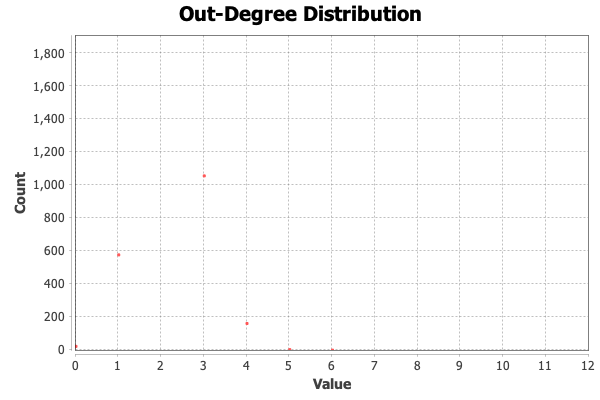
\includegraphics[scale=0.35]{images/2_1_outdegree-distribution.png}
	\end{tabular}
\end{table}

A continuación vamos a mostrar unas gráficas sobre tres medidas relacionadas con la distancia: \textit{Betweenness} (intermediación), \textit{Closeness} (cercanía) y \textit{Eccentricity} (excentricidad).

\begin{table}[H]
	\centering
	\begin{tabular}{ccc}
		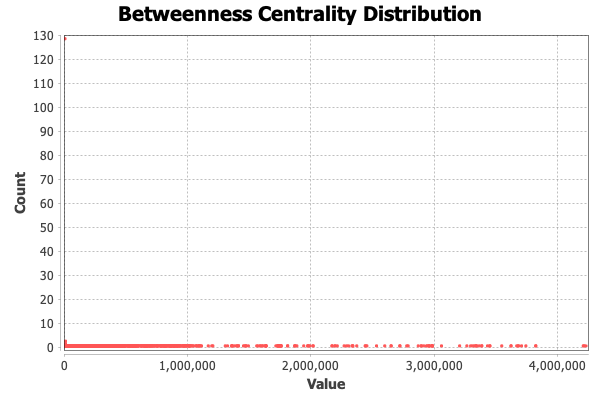
\includegraphics[scale=0.25]{images/2_1_betweenness.png} & 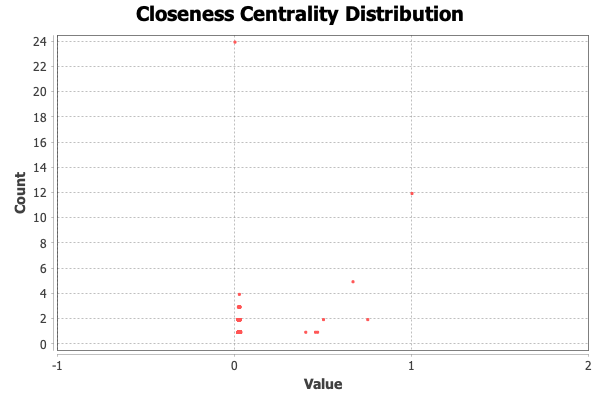
\includegraphics[scale=0.25]{images/2_1_closeness.png} &
		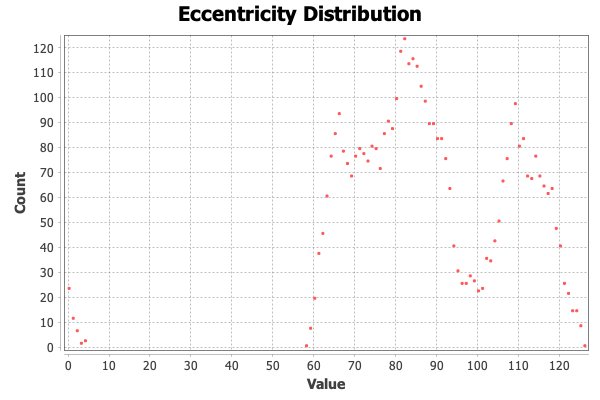
\includegraphics[scale=0.25]{images/2_1_eccentricity.png} 
	\end{tabular}
\end{table}

Otra gráfica de distancia interesante es la siguiente \footnote{La idea de representar estas dos medidas juntas ha sido sacada del paper (figura 3) de \textit{Renato Fabbri} nombrado en la bibliografía.}::

\begin{figure}[H]
	\centering
	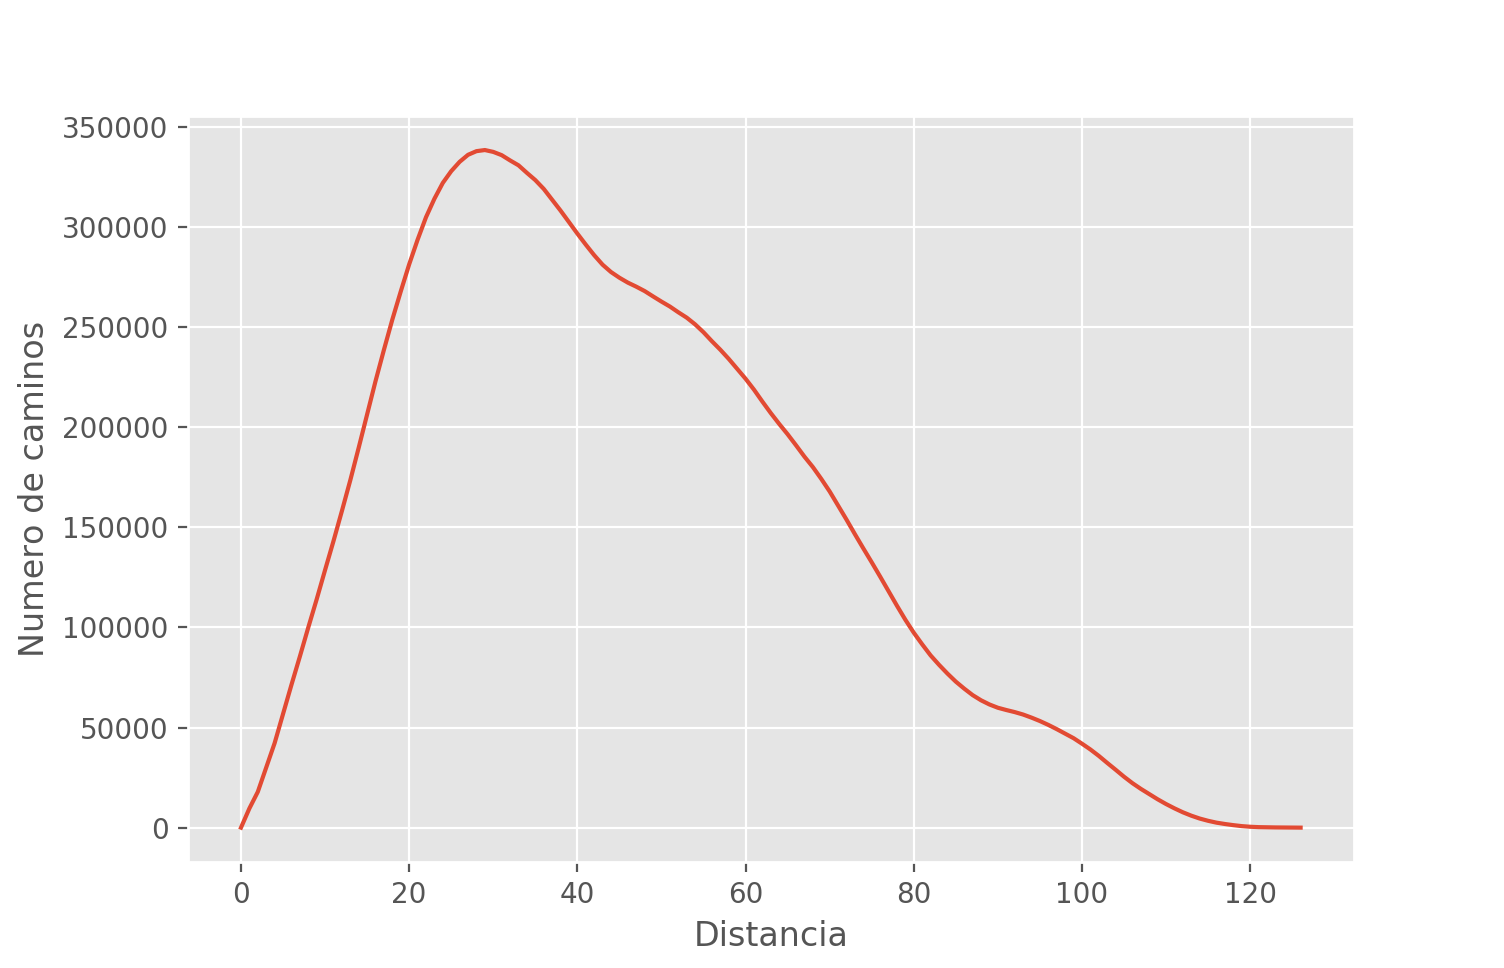
\includegraphics[scale=0.5]{images/2_1_distance.png}
\end{figure}

Finalmente, vamos a mostrar una gráfica sobre la distribución del grado de clustering:

\begin{figure}[H]
	\centering
	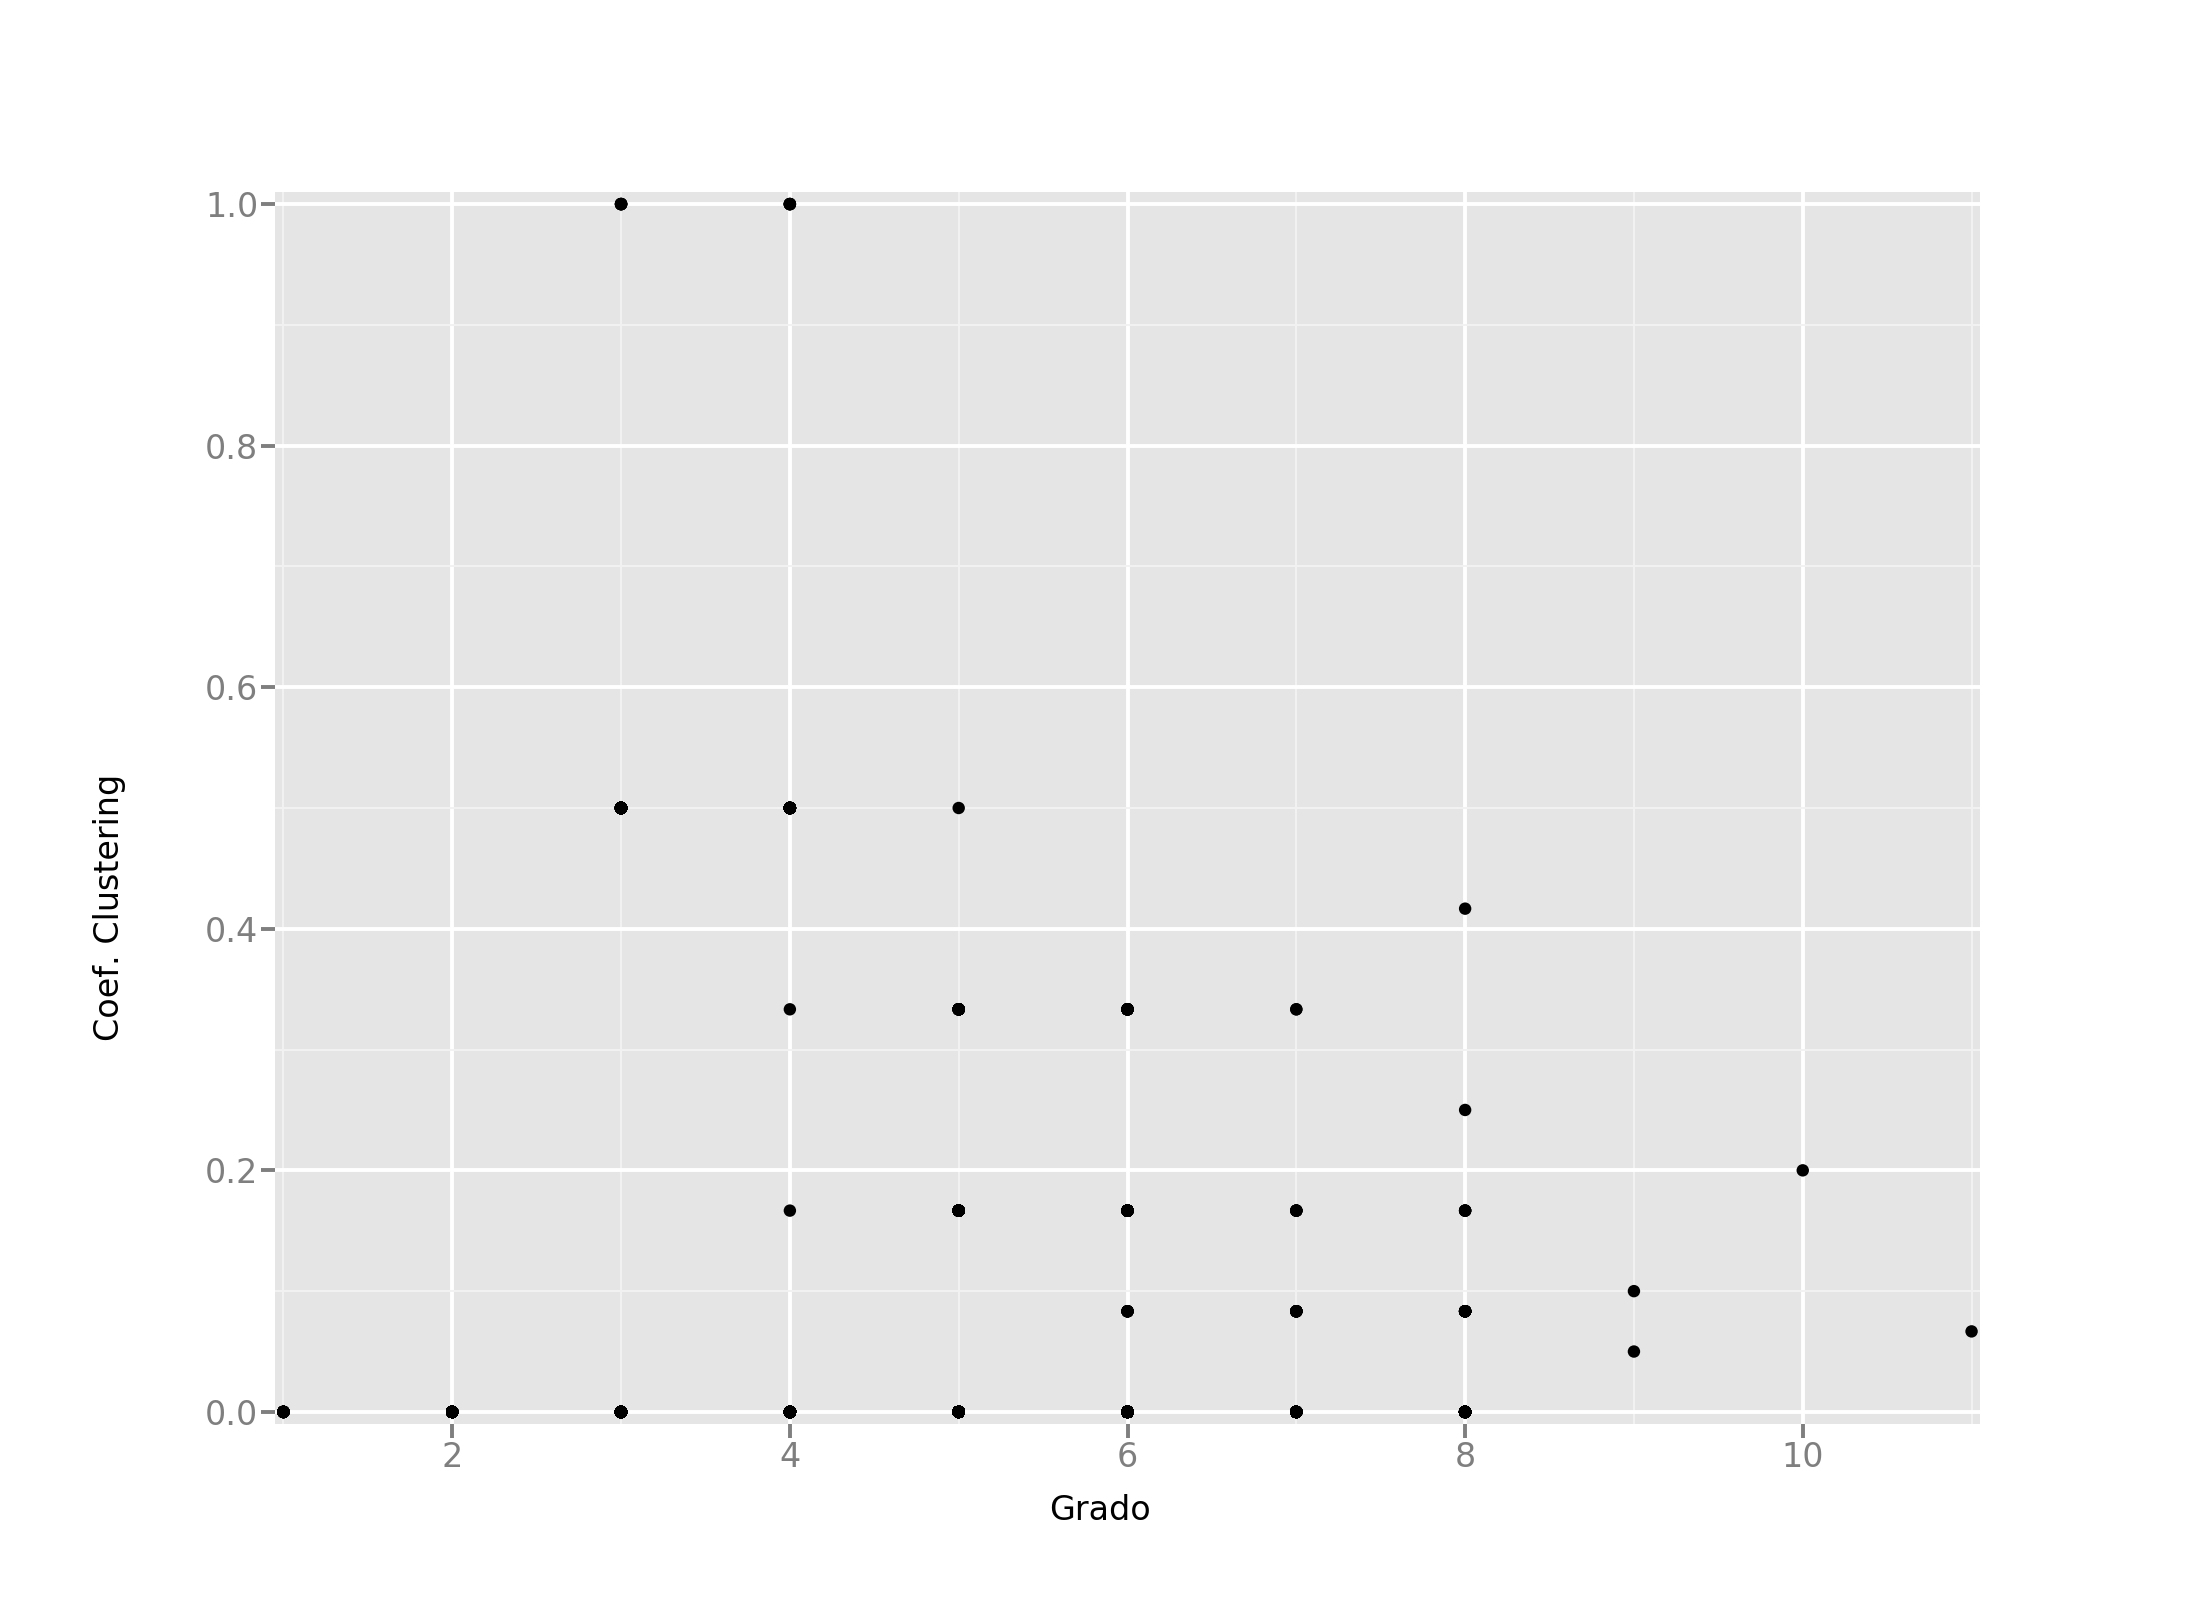
\includegraphics[scale=0.35]{images/2_1_clustering.png}
\end{figure}

Podemos concluir con un par de comentarios:

\begin{itemize}
	\item Las distribuciones de grados de nuestra red nos indican que esta no sigue la llamada ``Ley de la Potencia''. También podemos observar que no hay hubs claramente notables, ya que no hay una cantidad diferenciada de nodos con un grado más alto que los demás. 
	\item Si observamos la última gráfica de distancias, podemos ver que el mayor número de caminos lo tenemos para una distancia en torno a $30$. La gráfica no es simétrica del todo, por eso la distancia media es un poco más alta de $30$.
	\item Si observamos la gráfica de clustering, podemos ver que no hay muchos nodos con un alto coeficiente de clustering y con un grado alto. Esto nos hacer ver que las conexiones del área de Manhattan son bastante irregulares.
	\item Podemos ver que se trata de una red de mundo pequeño observando la gráfica de distancia. En dicha gráfica se representa el número de caminos de una distancia dada. Podemos ver que la mayoría de los caminos tienen una distancia pequeña, cercana a la distancia media. También vemos que el número de caminos que tiene una distancia grande son mínimos. Por lo tanto, podemos decir que estams ante una red de mundo pequeño.
\end{itemize}

\subsection{Estudio de la Centralidad de los Actores.}

Los cinco actores mas relevantes para cada medida son los siguientes:

\begin{table}[H]
	\centering
	\begin{tabular}{cccc}
		\textbf{\begin{tabular}[c]{@{}c@{}}Centralidad\\ de Grado\end{tabular}} & \textbf{\begin{tabular}[c]{@{}c@{}}Centralidad de\\ Intermediación\end{tabular}} & \textbf{\begin{tabular}[c]{@{}c@{}}Centralidad\\ de Cercanía\end{tabular}} & \textbf{\begin{tabular}[c]{@{}c@{}}Centralidad de\\ Vector propio\end{tabular}} \\ \hline
		2512378850: 11 & 42431099: 0.2168 & 486819531: 1 & 42427867: 1.0 \\
		42431257: 10 & 587812578: 0.2154 & 42423847: 1 & 42427870: 0.976 \\
		42429215: 9 & 42441382: 0.2148 & 371225088: 1 & 42437923: 0.964 \\
		42429226: 9 & 42441310: 0.2145 & 588455736: 1 & 42431242: 0.949 \\
		42422283: 8 & 42436719: 0.1948 &  3785586748: 1 & 42431252: 0.914
	\end{tabular}
\end{table}

\begin{itemize}
	\item Debemos tener cuidado con el grado, ya que como hemos visto en clase de teoría, se trata de una medida bastante local.
	\item La intermediación capta la correduría de la información por la estructura de la red. Obtiene un mayor valor para los nodos por los que pasen más caminos mínimos por él. Estos nodos son los que se encargan de hacer de puente entre comunidades y, por lo tanto, son usados para detectar comunidades.
	\item Como hemos visto en las transparencias de teoría, la cercanía es una forma de medir la centralidad, la cual plantea que el hecho de que puede no ser tan importante tener muchos amigos directos ni estar situado ``entre'' otros actores. En este caso, se le da importancia a ``estar en medio de las cosas'', no demasiado lejos del centro, para lo cual no es necesario estar en una posición de correduría. La suma de las distancias geodésicas (distancias de los caminos mínimos) para cada actor es la lejanía de dicho actor al resto. La inversa de dicha suma es la medida de cercanía.
	\item La centralidad de vector propio tiene como base la idea de que la centralidad de un nodo depende de cómo de centrales sean sus nodos vecinos. La idea es que el poder y el status de un actor (ego) se define recursivamente a partir del poder y el status de sus vecinos (alters). Es una versión más elaborada de la centralidad de grado al asumir que no todas las conexiones tienen la misma importancia. Es como dice el dicho, ``más vale calidad que cantidad''.
\end{itemize}

A continuación voy a mostrar la red destacando las medidas estudiadas en esta sección. Para ello, he aplicado el algoritmo \textit{Fruchterman Reingold} para poder visualizar la red de una forma más práctica. A continuación, se ha cambiado el tamaño y el color de los nodos para representar las distintas métricas: a mayor tamaño y más oscuro es el color verde, mayor es la medida representada. Quiero remarcar un aspecto interesante, la medida de grado está bastante repartida, es decir, no hay nodos que destaquen. Podemos ver como en las otras tres representaciones si hay nodos más destacados, sobre todo en la medida de centralidad de vector propio.

\begin{figure}[H]
	\centering
	\subfloat[Centralidad de grado.]{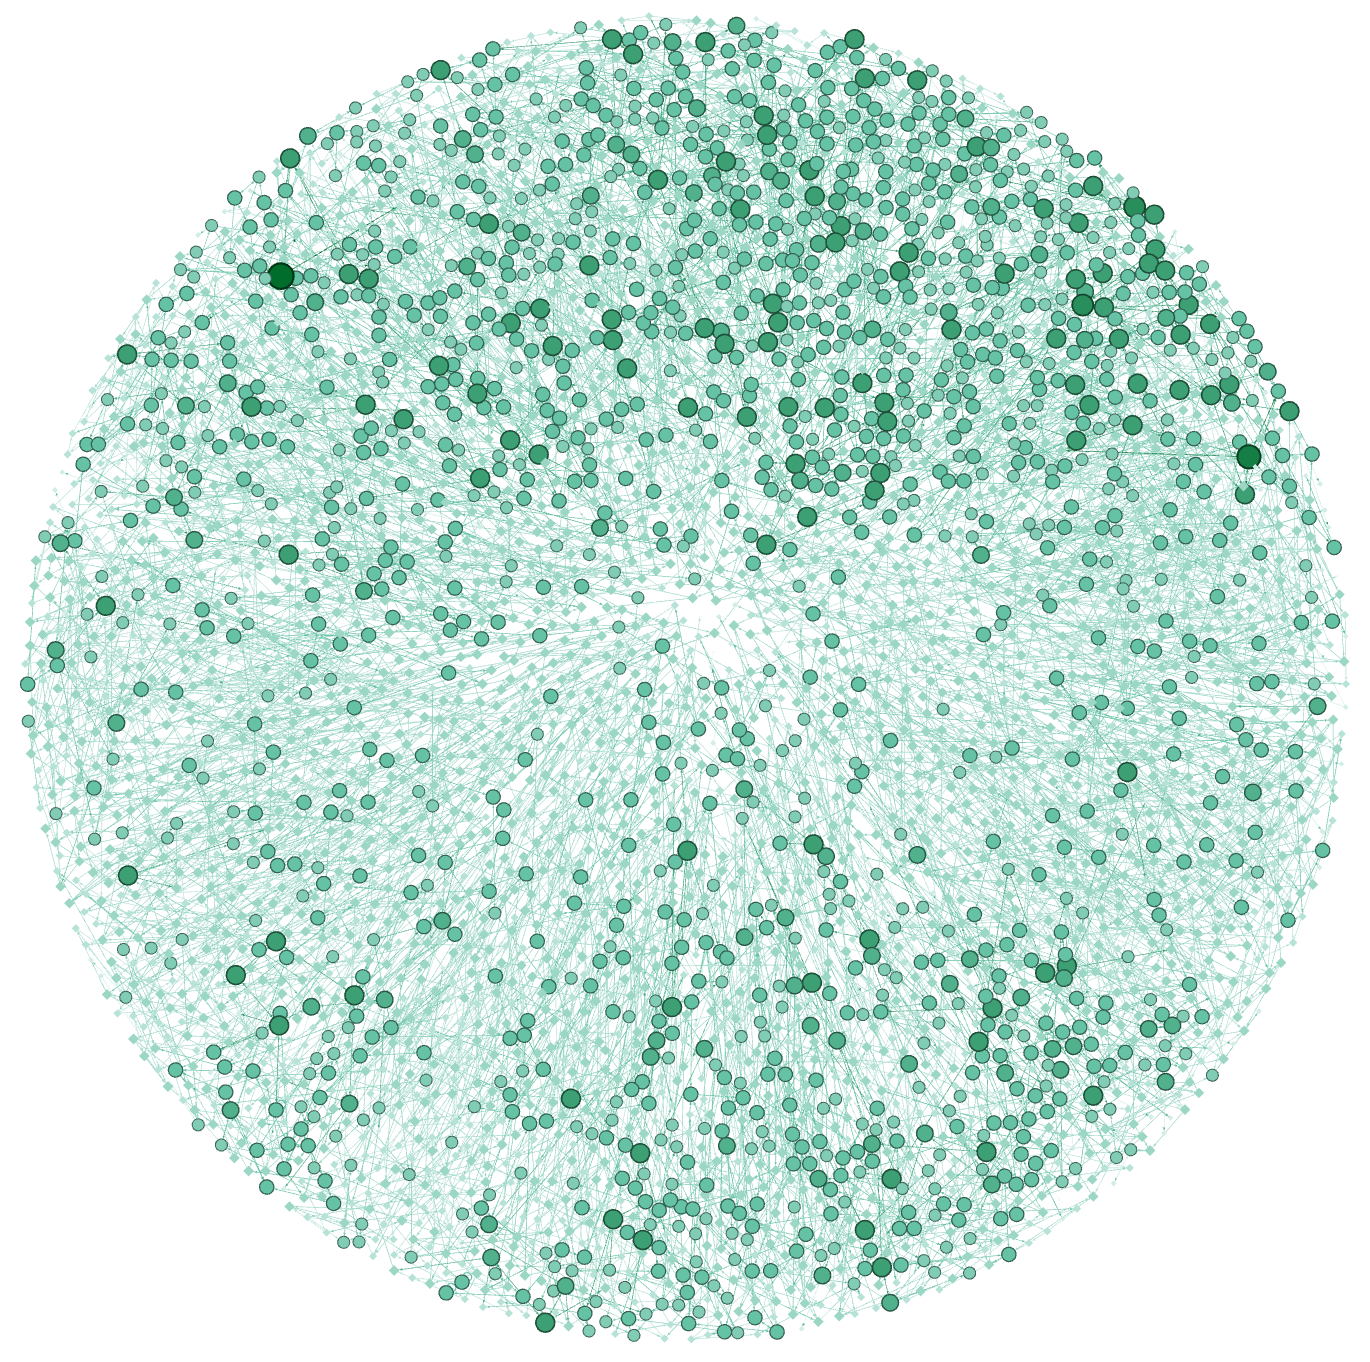
\includegraphics[width=0.5\textwidth]{images/2_2_degree.png}}
	\subfloat[Centralidad de intermediación.]{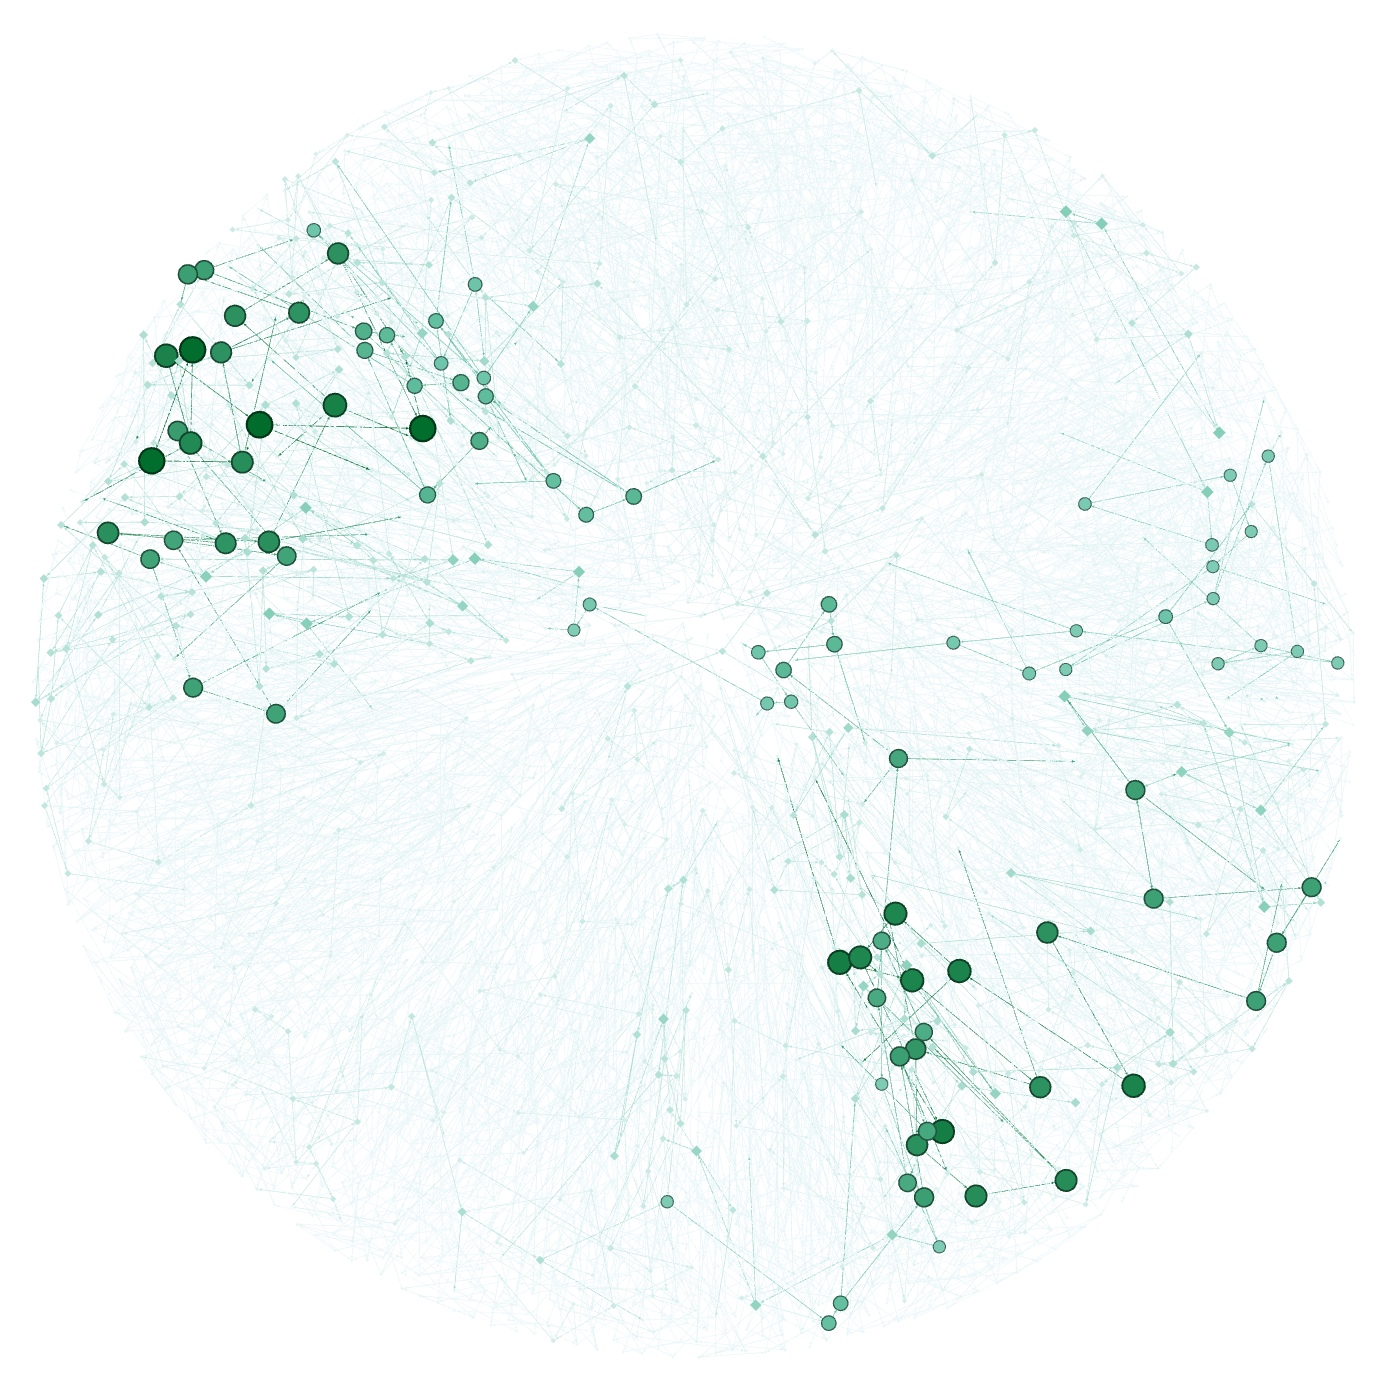
\includegraphics[width=0.5\textwidth]{images/2_2_betweenness.png}} \\
	\subfloat[Centralidad de cercanía.]{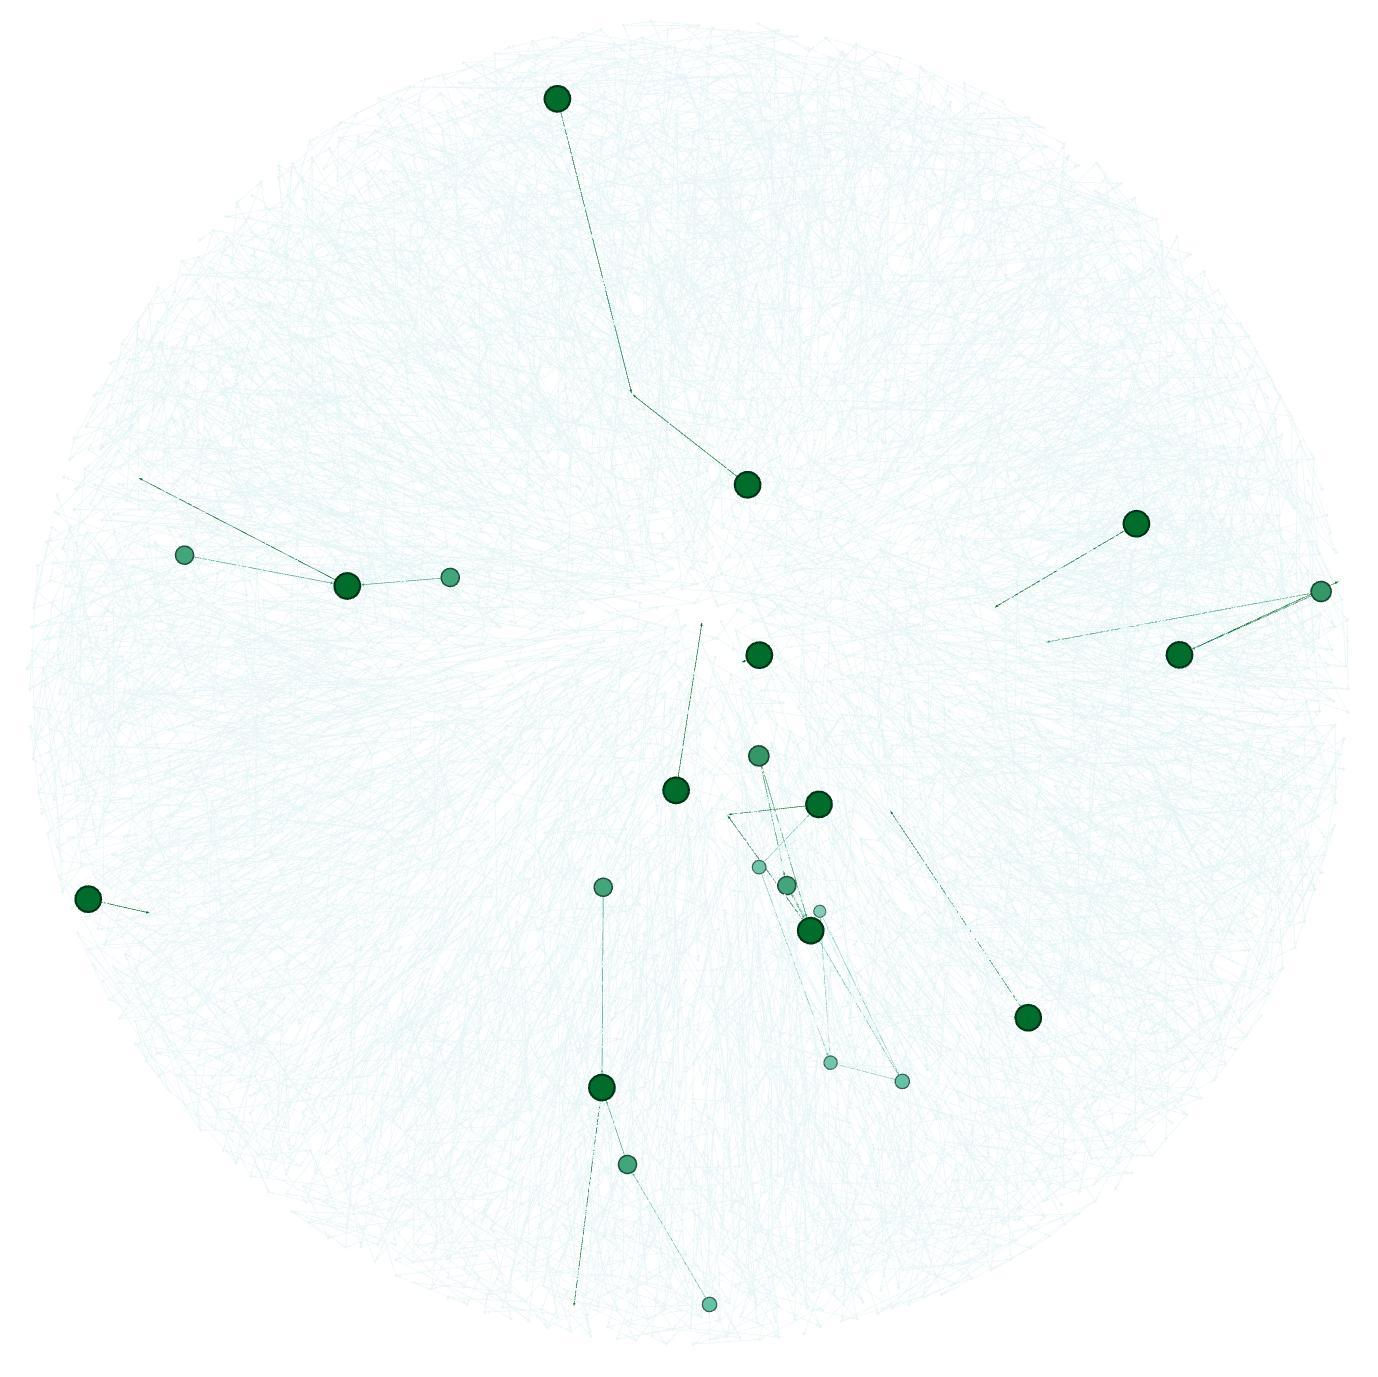
\includegraphics[width=0.5\textwidth]{images/2_2_closeness.png}}
	\subfloat[Centralidad de vector propio.]{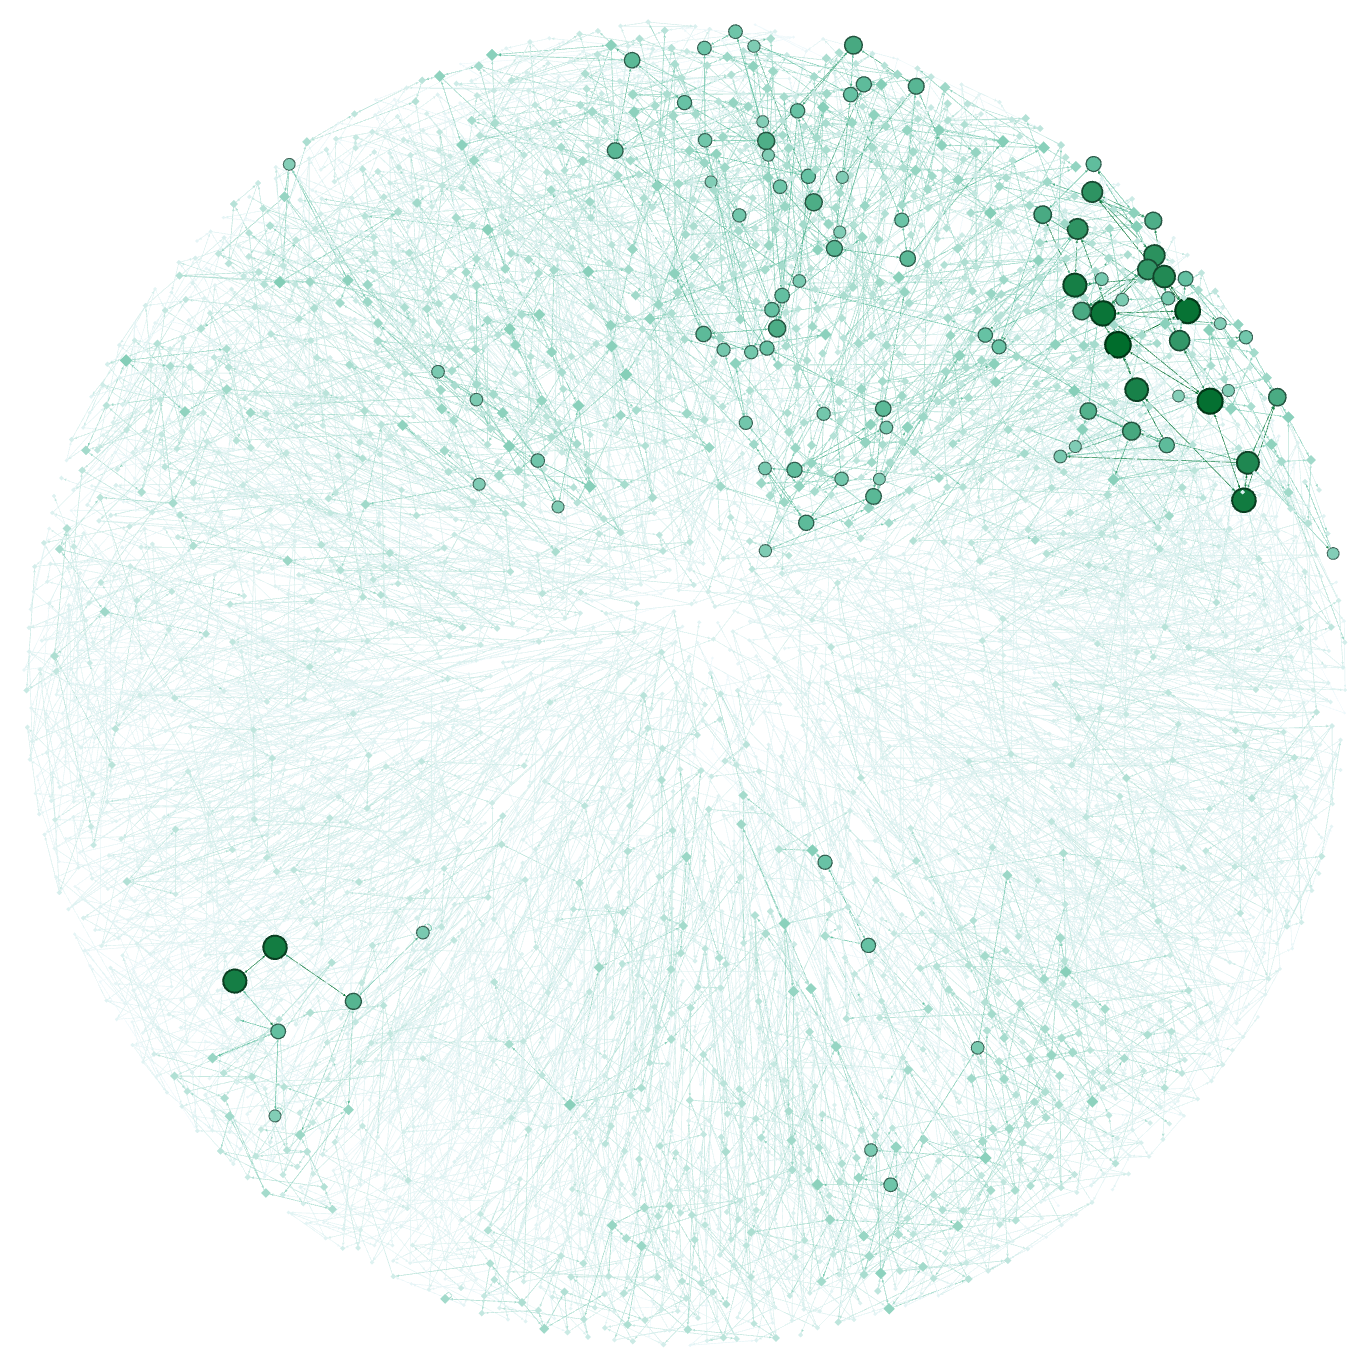
\includegraphics[width=0.5\textwidth]{images/2_2_eigenvector.png}}
\end{figure}

Finalmente, tal y como se indica en el guión de prácticas, vamos a mostrar una gráfica en la que se visualicaz dos de las medidas anteriores, la intermediación en el tamaño de los nodos y la centralidad de vector propio en el color de los mismos:

\begin{figure}[H]
	\centering
	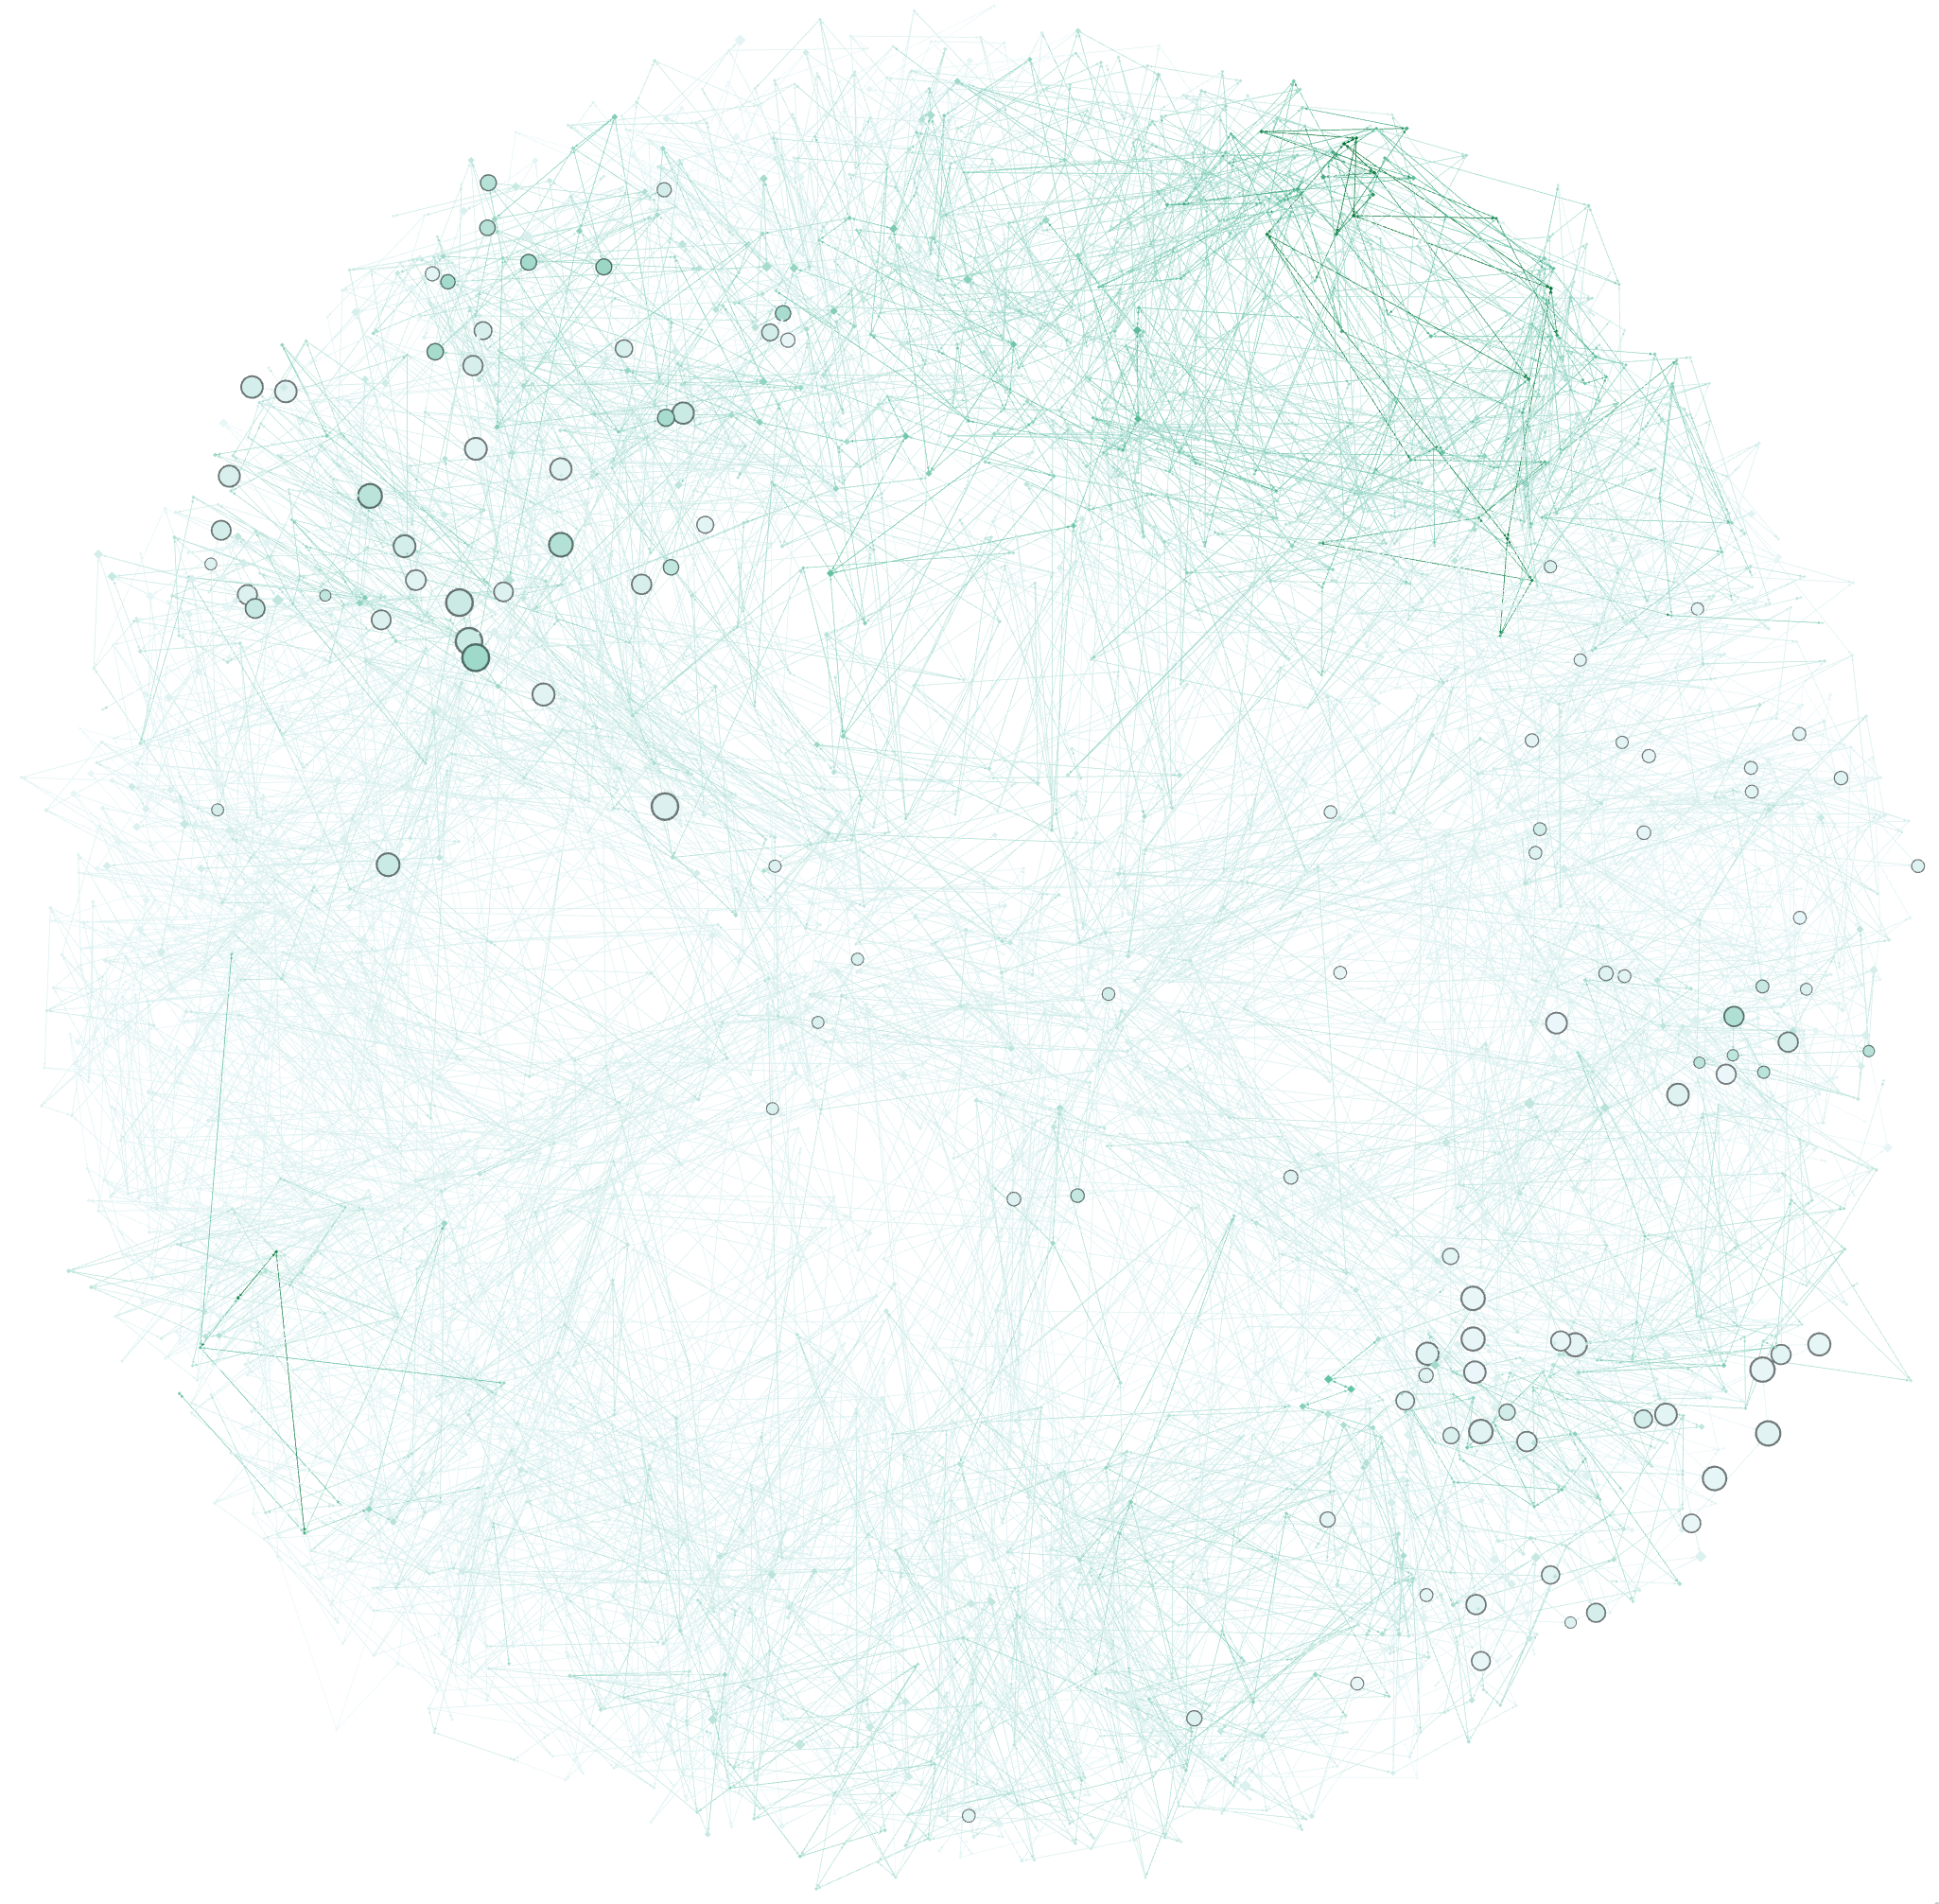
\includegraphics[width=0.6\linewidth]{images/2_2_betweenness_eigenvector.png}
\end{figure}

Cómo podemos ver, hay nodos en los que ambas medidas coinciden, como puede ser la zona de la izquierda donde se ven los nodos más grandes. Sin embargo, en la zona superior derecha, podemos ver que los nodos tienen un alto valor de la centralidad de vector propio (nodos muy oscuros) pero una intermediación bastante pequeña (nodos muy pequeños). \\

Finalmente, vamos a mostrar un gráfico que representa los valores de dos de las medidas para todos los actores de la red en ejes de coordenadas como los estudiados en la Sesión I.2. En mi caso, voy a representar las mismas medidas que he mostrado en el gráfico anterior:

\begin{figure}[H]
	\centering
	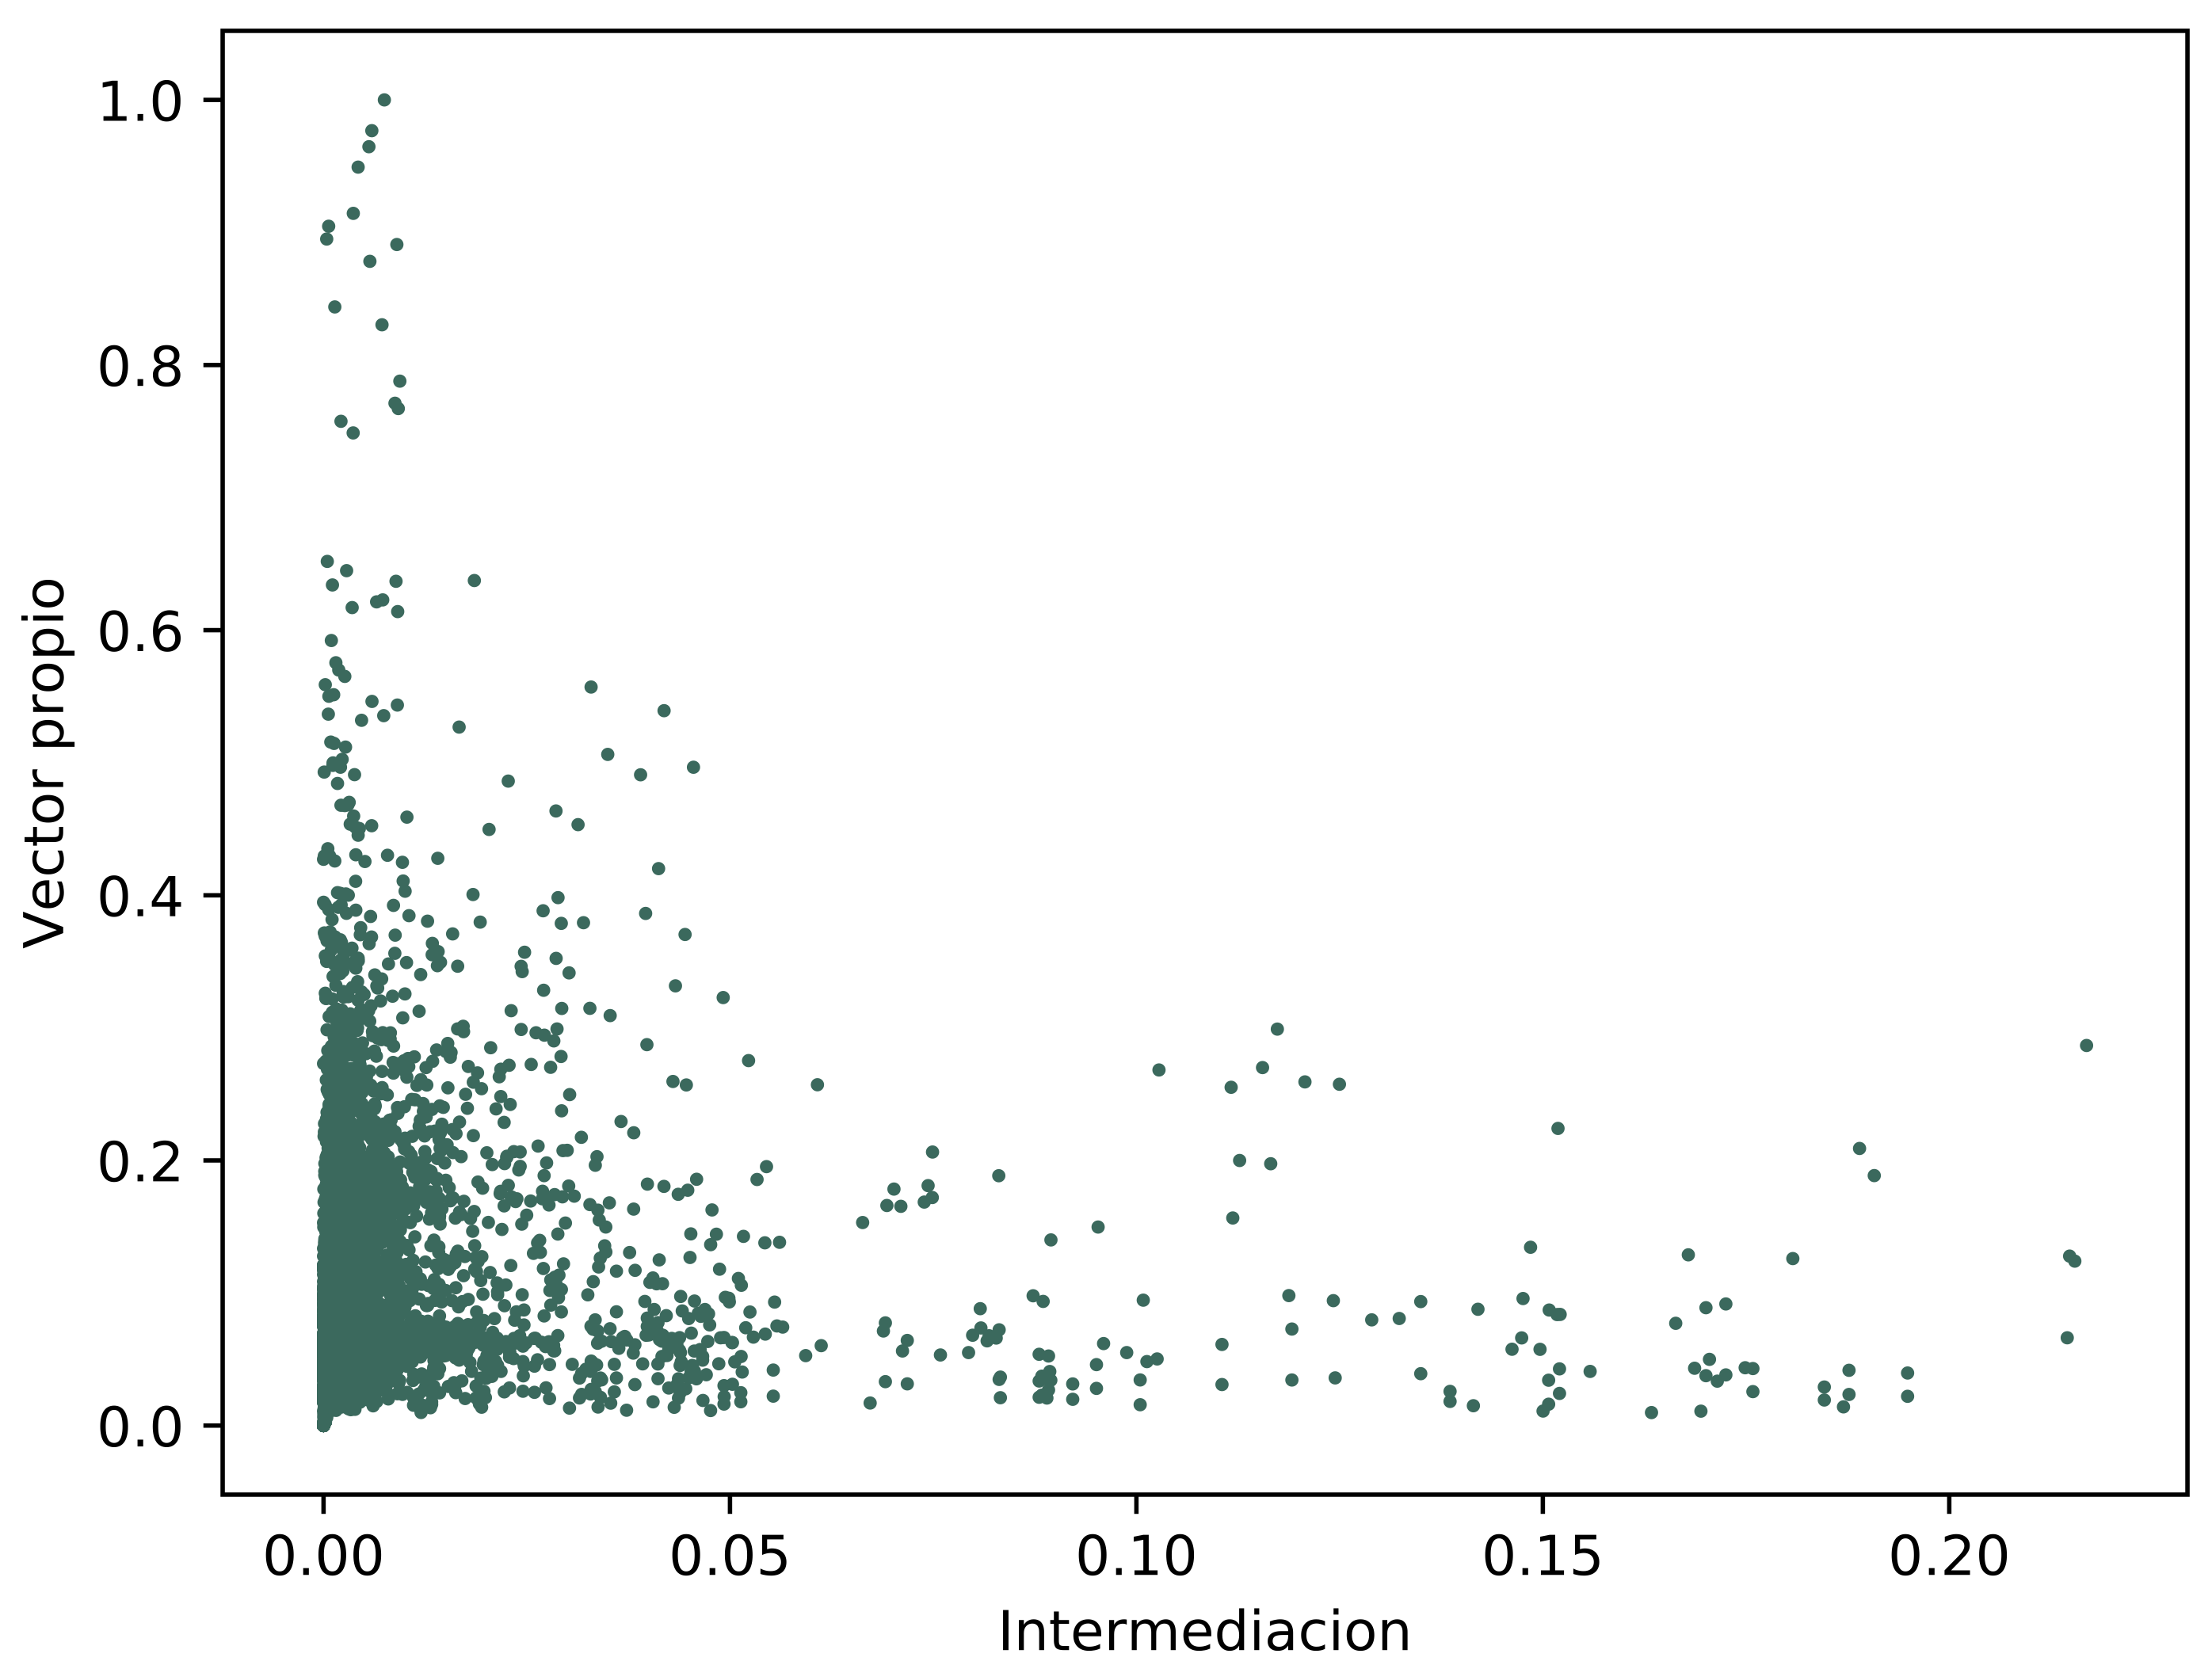
\includegraphics[width=0.6\linewidth]{images/2_2_betweenness_eigenvector_axis.png}
\end{figure}

Como podemos ver, la mayoría de los nodos tienen un valor de vector propio muy bajo y un valor de intermediación muy bajo. También podemos ver que los nodos que tienen un valor alto de vector propio tiene un valor bajo de intermediación y viceversa. 

\subsection{Detección de Comunidades.}

Para la detección de comunidades se ha aplicado el método de \textit{Lovaina} con distintos valores para el parámetro resolución. Los resultados obtenidos son los siguientes:

\begin{figure}[H]
	\centering
	\subfloat[Resolución: 1.0.]{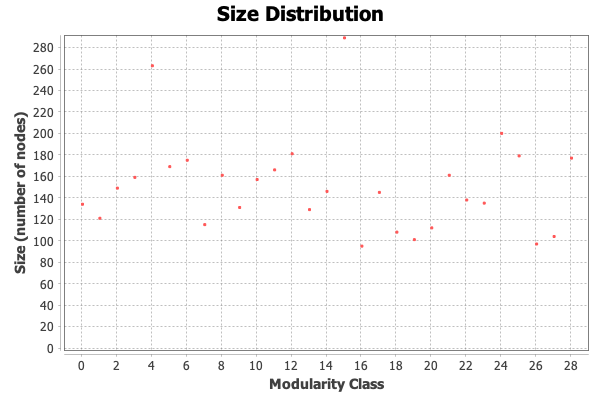
\includegraphics[width=0.3\textwidth]{images/2_3_1_communities-size-distribution.png}}
	\subfloat[Resolución: 5.0.]{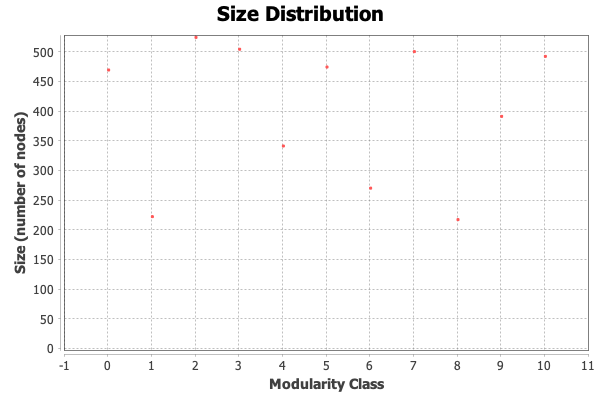
\includegraphics[width=0.3\textwidth]{images/2_3_5_communities-size-distribution.png}}
	\subfloat[Resolución: 10.0.]{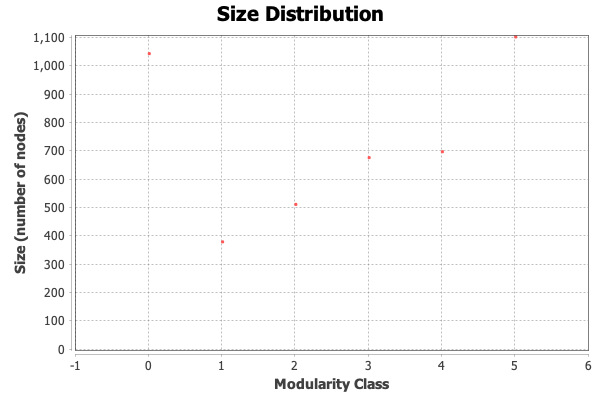
\includegraphics[width=0.3\textwidth]{images/2_3_10_communities-size-distribution.png}}
\end{figure}

\begin{table}[H]
	\centering
	\begin{tabular}{cccc}
		\textbf{Resolución} & \textbf{\begin{tabular}[c]{@{}c@{}}Número de \\ comunidades\end{tabular}} & \textbf{Modularidad} & \textbf{\begin{tabular}[c]{@{}c@{}}Modularidad \\ con resolución\end{tabular}} \\ \hline
		1.0 & 29 & 0.906 & 0.906 \\
		5.0 & 11 & 0.874 & 4.764 \\
		10.0 & 6 & 0.797 & 9.662
	\end{tabular}
\end{table}

Cómo podemos ver, aumentar el valor de resolución supone reducir el número de comunidad y, por lo tanto, reducir el valor de la modularidad. A su vez, aumenta la modularidad con resolución de la red. A continuación, voy a mostrar unas imágenes que representan la red en función de la comunidad a la que pertenecen. Primero vamos a ver los resultados obtenidos para una resolución de \textit{1.0}:

\begin{figure}[H]
	\centering
	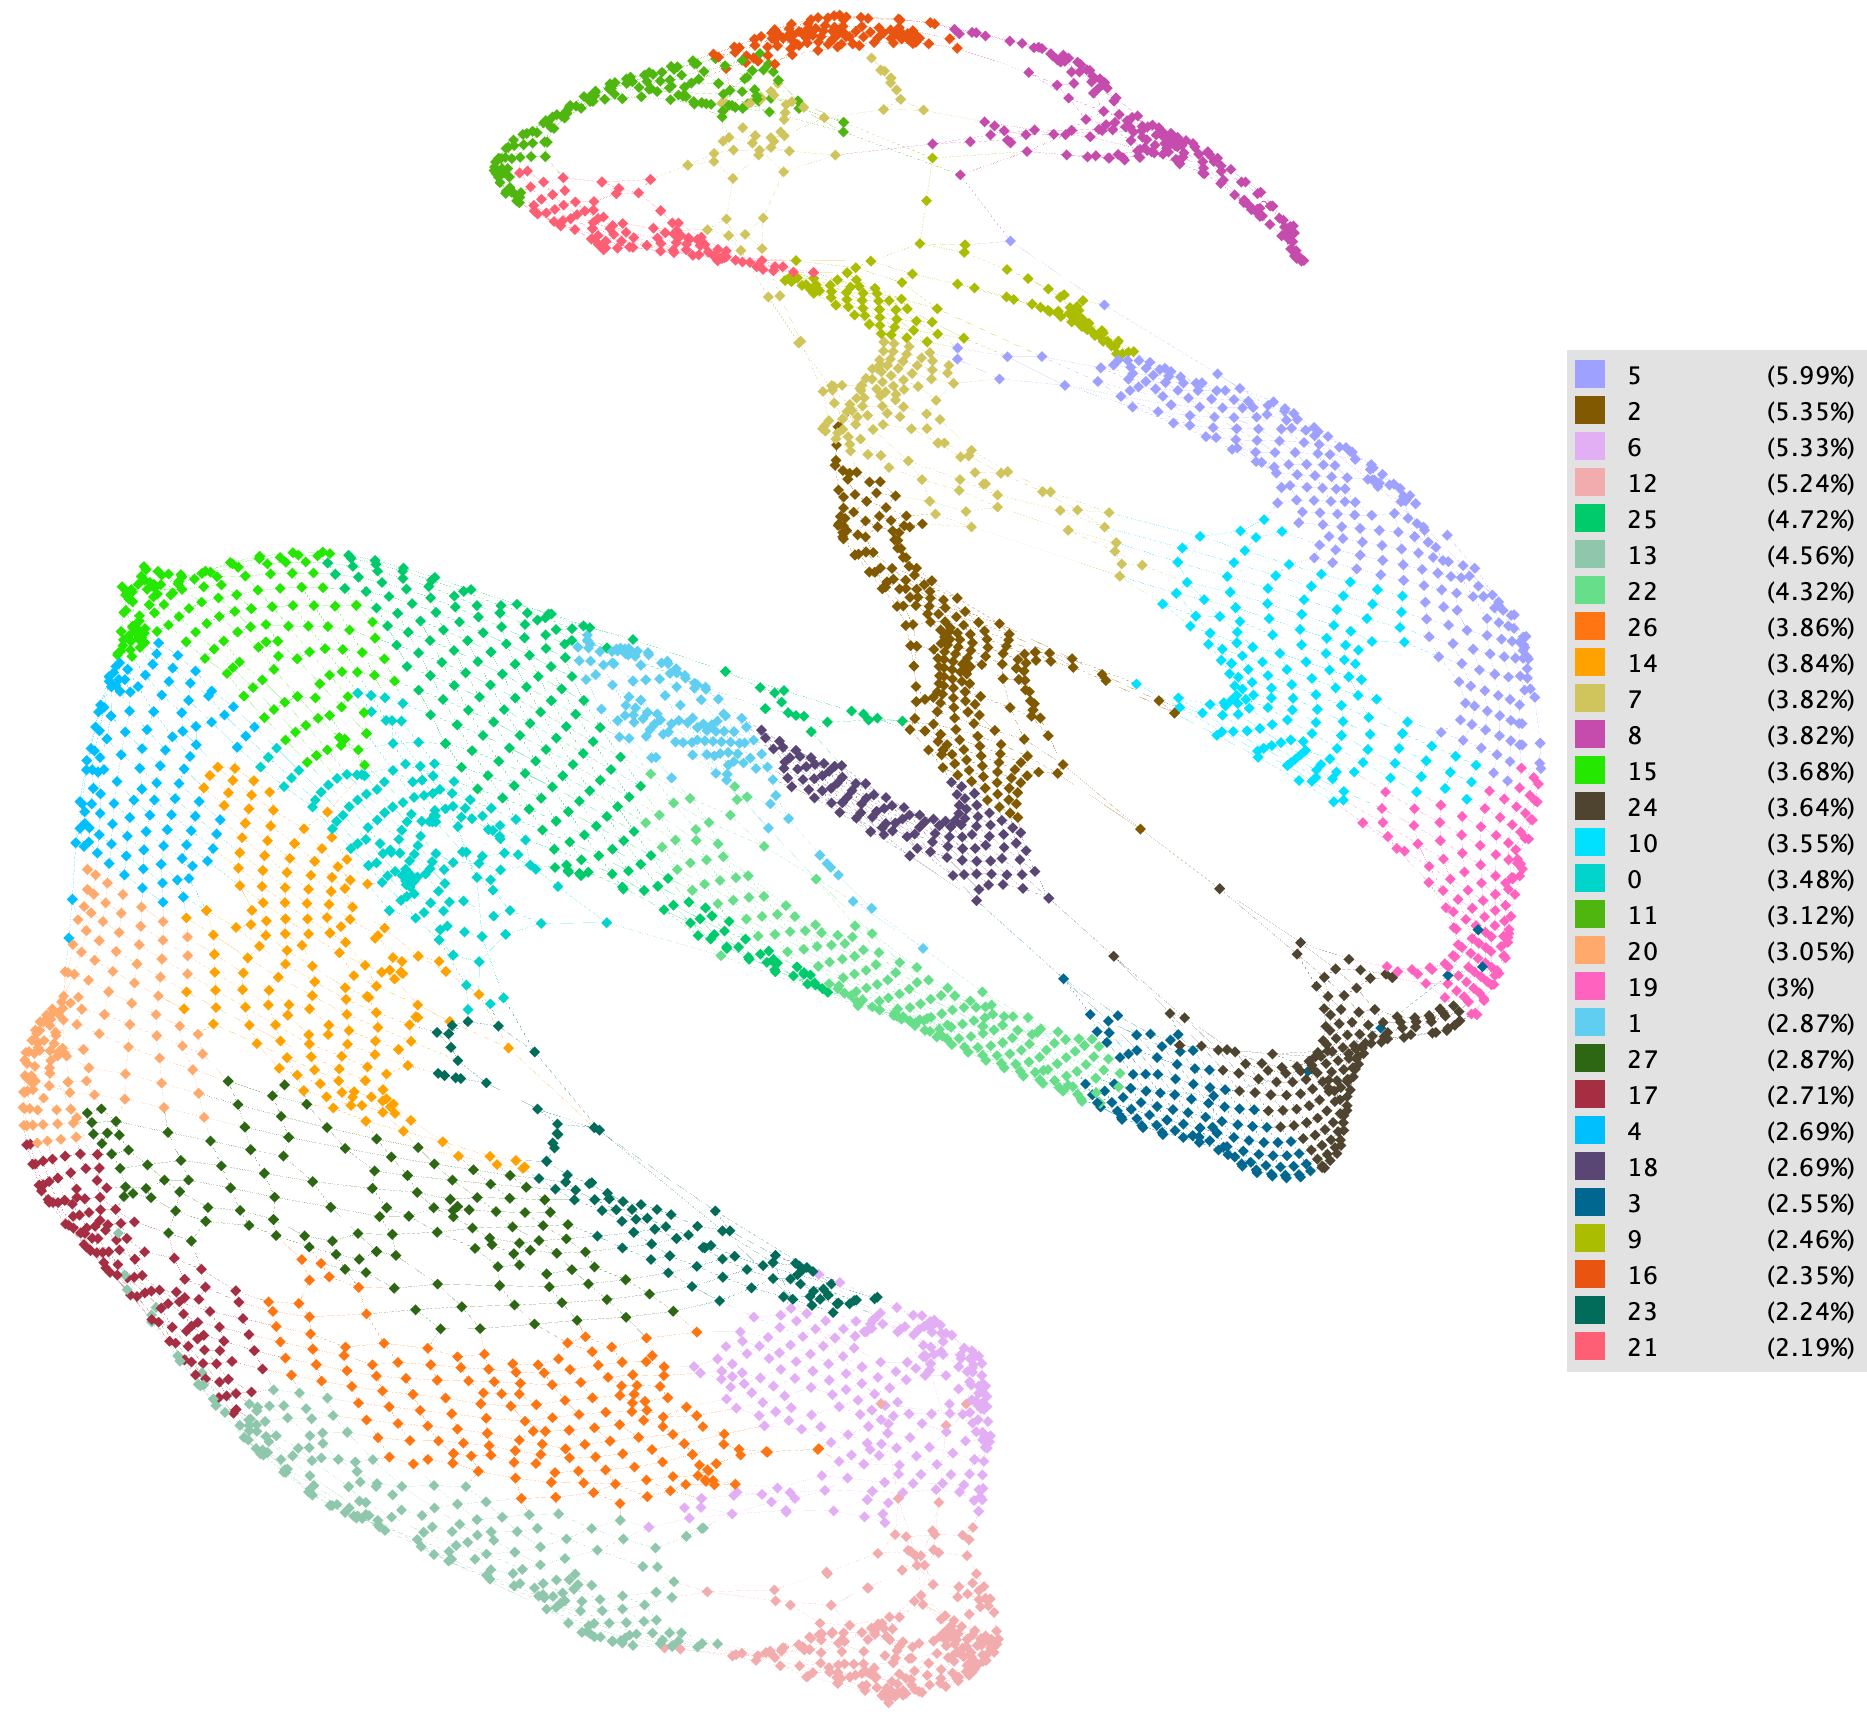
\includegraphics[width=\linewidth]{images/2_3_1_lovaina.png}
\end{figure}

A continuación, vamos a ver los resultados obtenidos para una resolución de \textit{5.0}:

\begin{figure}[H]
	\centering
	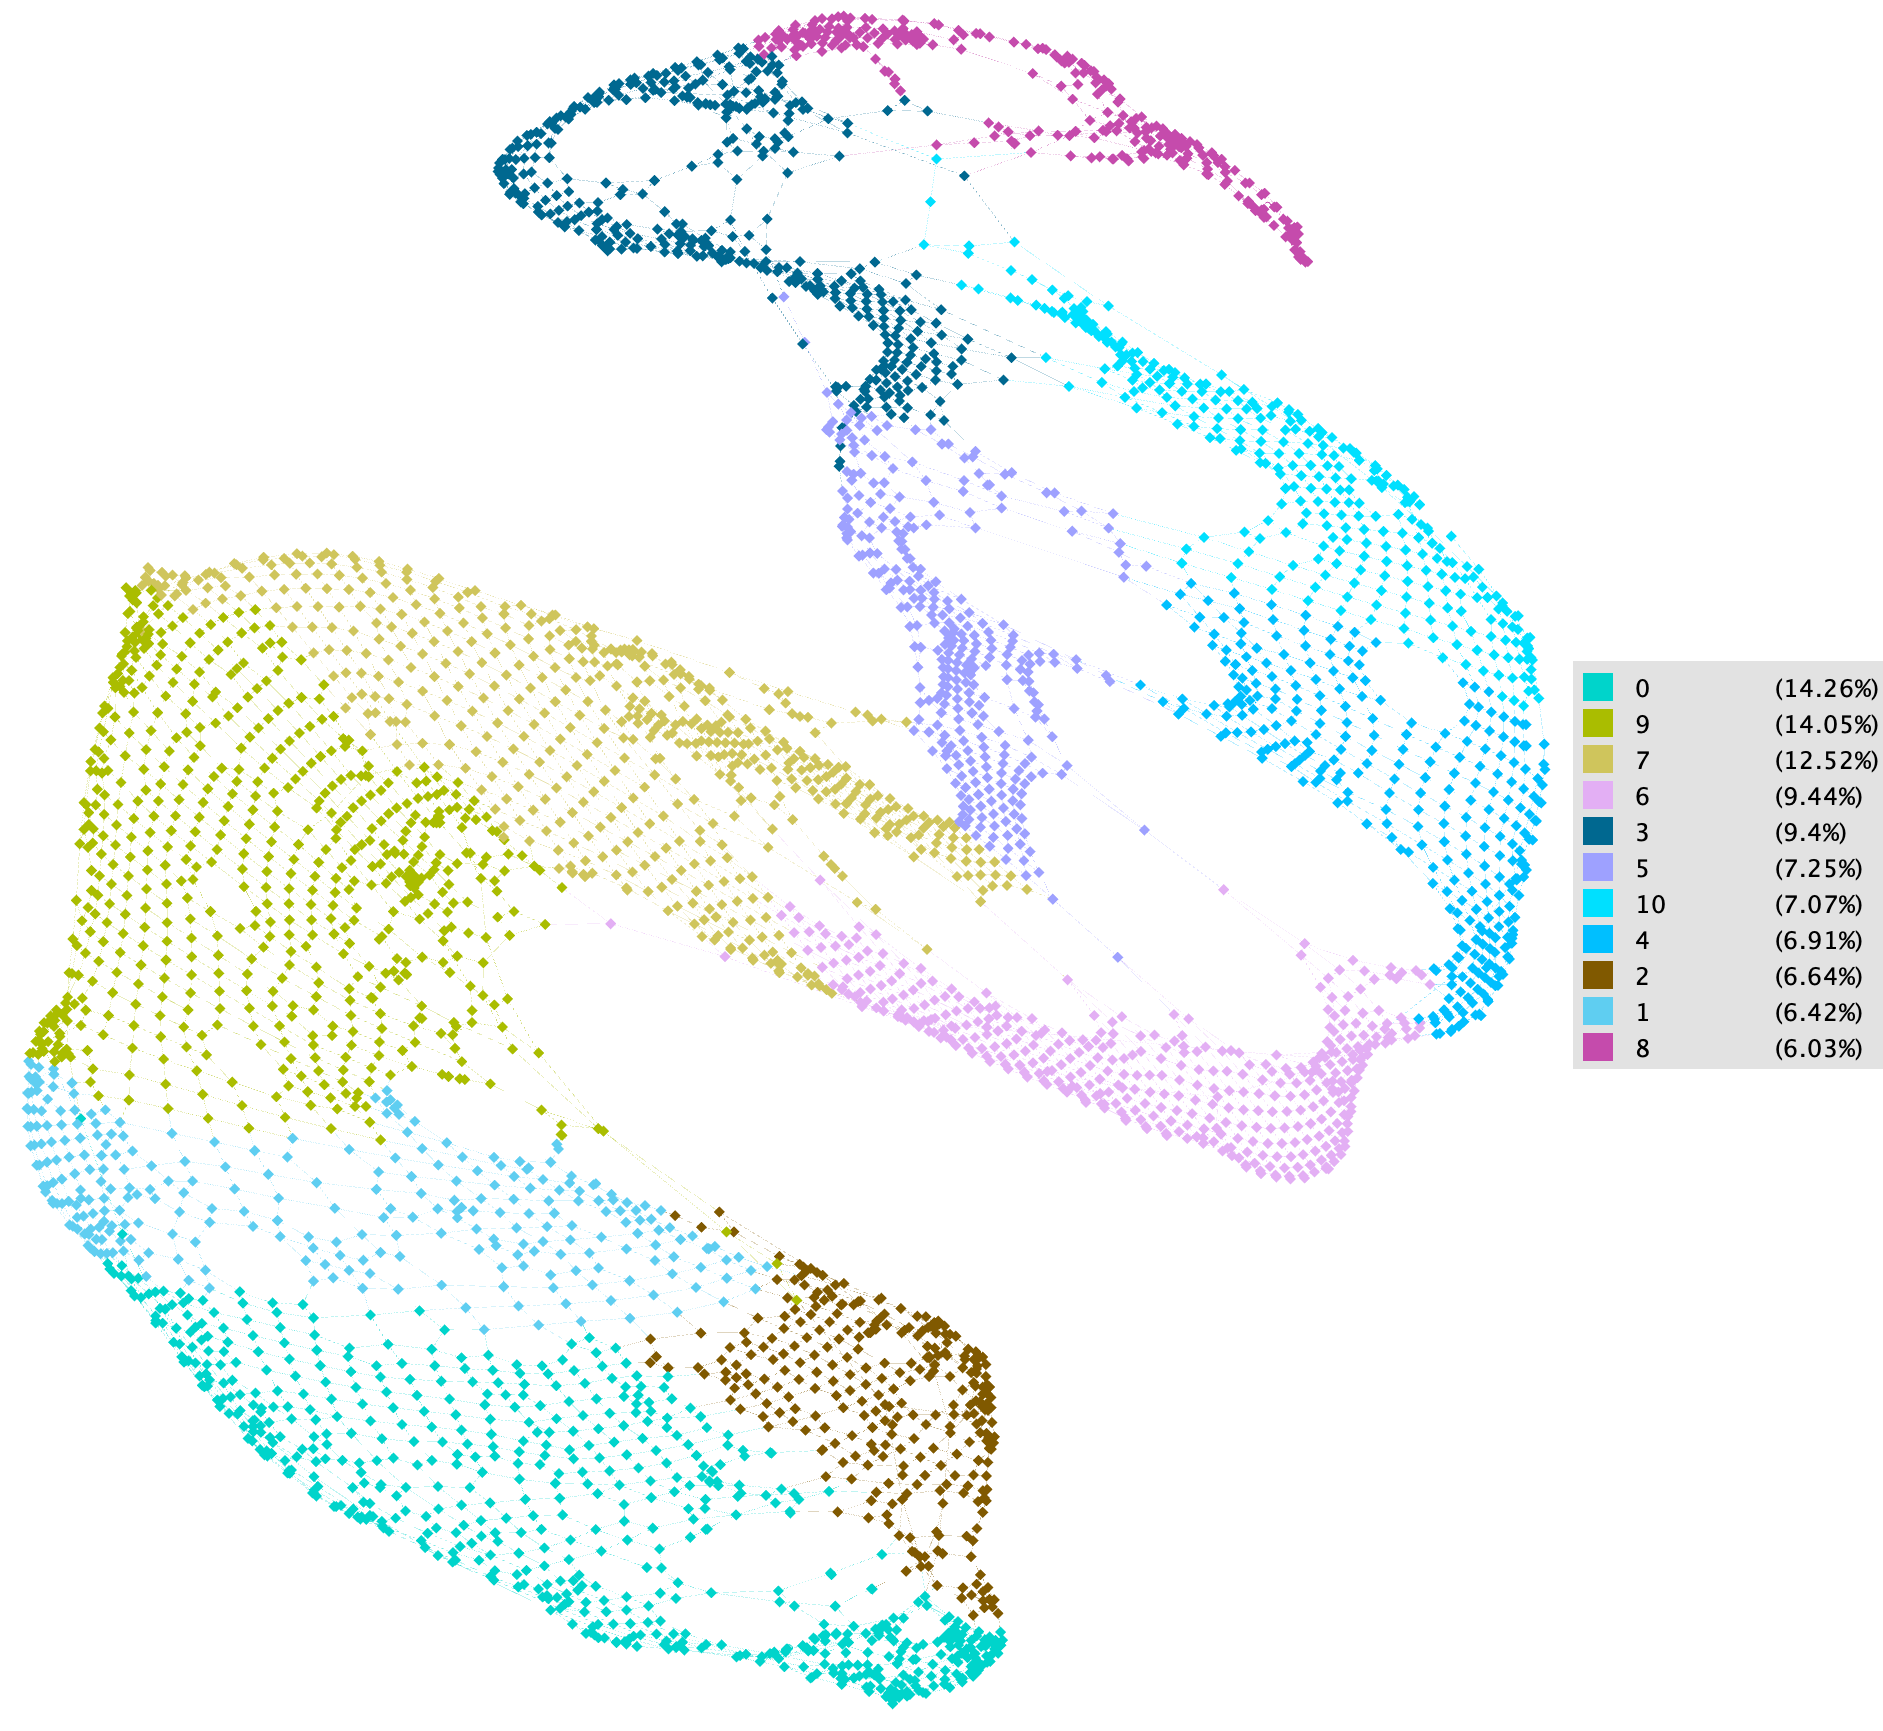
\includegraphics[width=\linewidth]{images/2_3_5_lovaina.png}
\end{figure}

Finalmente, vamos a ver los resultados obtenidos para una resolución de \textit{10.0}:

\begin{figure}[H]
	\centering
	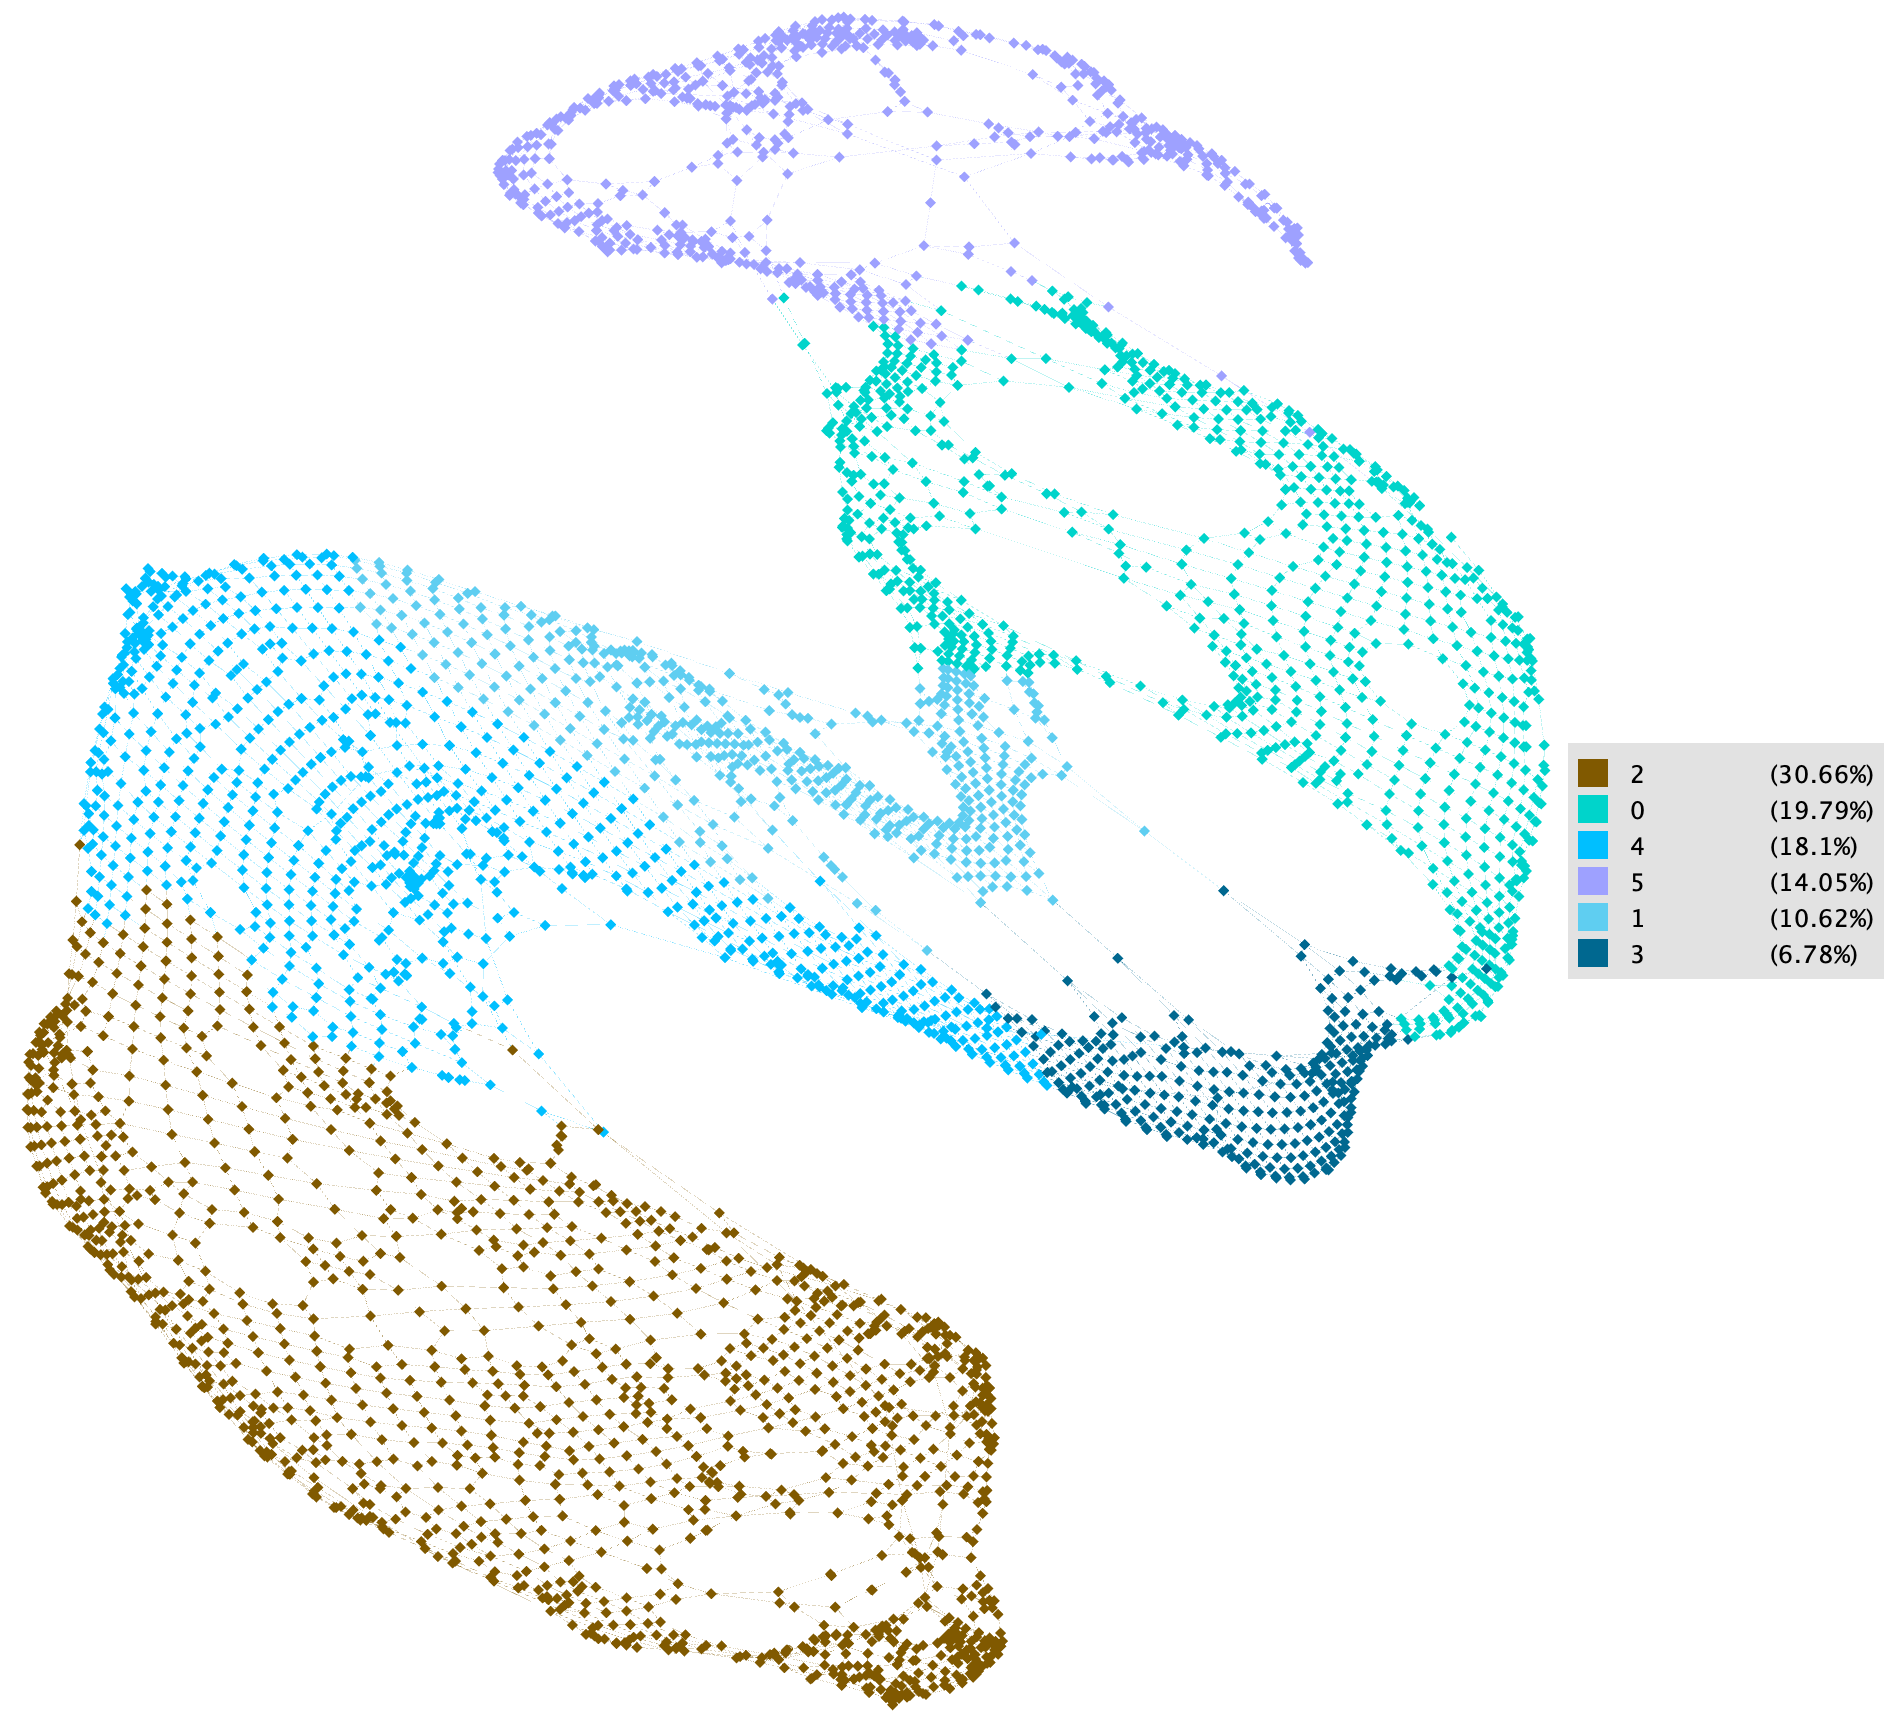
\includegraphics[width=\linewidth]{images/2_3_10_lovaina.png}
\end{figure}

Para la visualización de las comunidades he usado el algoritmo \textit{Force Atlas 2}, ya que permite ver con mucha claridad las comunidades detectadas en la red. Como podemos ver, no hay comunidades claras como hemos estudiado en la asignatura, ya que ninguna frontera de las mismas es totalmente clara. Sin embargo, podemos ver como las comunidades representan zonas contiguas de Manhattan. En el problema concreto que estamos estudiando, esta idea de comunidades se podría utilizar para definir zonas por las cuales se pueden mover los taxis y poner un precio al servicio según la zona en la que se mueven o según la zona de origen y destino.

\subsection{Gráficos adicionales.}

Los gráficos adicionales se han mostrado a lo largo de la memoria en su sección correspondiente.

\section{Bibliografía.}

\begin{itemize}
	\item \href{https://networkx.github.io}{networkx}: Herramienta usada para realizar ciertas gráficas.
	\item \href{https://graph-tool.skewed.de}{graph-tool}: Herramienta usada para realizar ciertas gráficas.
	\item \href{https://www.researchgate.net/publication/258114132_On_the_evolution_of_interaction_networks_primitive_typology_of_vertex_and_prominence_of_measures}{On the evolution of interaction networks: primitive typology of vertex and prominence of measures - Renato Fabbri, Vilson Vieira da Silva Junior, Ricardo Fabbri y Osvaldo N Oliveira} 
	\item \href{https://gephi.org/}{Gephi}.
\end{itemize}

\end{document}